\documentclass[a4,12pt]{book}
\usepackage{amsmath,amssymb}

\usepackage{geometry}
\geometry{
textwidth=157mm,
paperwidth=196mm,
paperheight=280mm,
top=1in,
left=27mm,
footskip=.7in
}

% Para enumerates customizados
\usepackage{enumerate}

% Para usar tabelas balanceadas
\usepackage{tabulary}

% Place crop marks
\usepackage[center,height=297mm,width=210mm,cam]{crop}

% Choose font
\usepackage{ifxetex}
\ifxetex
   \usepackage{fontspec}
   \setmainfont{Lato Light}
   \newfontface\titlefont{STIXIntegralsUp}
   \newfontface\thickfont{Nimbus Sans L}
   \newfontface\bigtitlefont[Scale=1.3]{Cabin}
   %\newcommand\titlefont{}
   %\newcommand\thickfont{}
\else
   \usepackage[utf8]{inputenc}
   \usepackage[sfdefault,thin]{roboto}  %% sfdefault is the base font
   \newcommand\titlefont{\fontfamily{helvet}\selectfont}
   \newcommand\thickfont{\fontfamily{cmss}\selectfont}
   \newcommand\bigtitlefont{\fontfamily{cmss}\selectfont}
\fi

% Larger spacing between lines
\linespread{1.2}

% Temporary library for generating random text
\usepackage{lipsum}

% To define colors
\usepackage[dvipsnames]{xcolor}
\definecolor{titleblue}{RGB}{21,101,175}
\definecolor{myblue}{RGB}{204,216,241}
\definecolor{mediumblue}{RGB}{108,153,215}
\definecolor{myred}{RGB}{210,32,39}
\definecolor{mygreen}{RGB}{179,220,47}


% use o GIMP para obter o cógigo HTML da cor e o site a seguir para converter para RGB
% http://www.yellowpipe.com/yis/tools/hex-to-rgb/color-converter.php


% \usepackage{lastpage} % Required to determine the last page for the footer

% Pacotes para desenhos
\usepackage{tikz}
\usetikzlibrary{shapes}
\usetikzlibrary{calc}
% This package provides special PGF/TikZ nodes for the text, marginpar, footer and header area of the current page.
\usepackage{tikzpagenodes}
\tikzset{x=1mm,y=1mm}

%%%%%%%%%%%%%%%%%%%% Chapter and section titles %%%%%%%%%%%%%%%%%%%%%%%%%
\usepackage[explicit]{titlesec} % needed for define chapter and section style.
\setcounter{chapter}{1}
%%%%%%%%%%%%%%%%%%%%%%%%%%%%%%%%%%%%%%%%%%%%%%%%%%%%%%
\usepackage{titling}

% Chapter
\titleformat{\chapter} % redefining chapter appearence
%{} % style
{\titlefont\Huge\bf} % style
{} % label
{0pt} % separation
{\begin{tikzpicture}[remember picture,overlay]
    \filldraw [x=1mm,y=1mm, mygreen, overlay] (37,0) circle [radius=9];
    \filldraw [x=1mm,y=1mm, myred, overlay] (58,0) circle [radius=9];
    \filldraw [x=1mm,y=1mm, titleblue, overlay] (79,0) circle [radius=9];
    \filldraw [x=1mm,y=1mm, mediumblue, overlay] (210,-9) -- (100 ,-9) arc (-90:-270:9) --(100,9)
    -- (210,9) (118, 0) node{\color{white} Lição \thechapter} (105,-27);
  \end{tikzpicture}
} % before title
[\vspace{3cm} \hfill {\bf\bigtitlefont \color{mygreen} #1}] % after title
%\titlespacing*{\chapter}{0pt}{50pt}{100pt} % {<command>}{<left>}{<before-sep>}{<after-sep>}

% Section style %%%%%%%%%%%%%%%%%%%%%%%%%%%%%%%%
%\newcommand*\sectionlabel{}
\titleformat{\section}
  {\titlefont\bf}
  {\gdef\sectionlabel{\thesection\ }}{0pt}
  {%
    \begin{tikzpicture}[remember picture,overlay]
      \filldraw [x=1mm,y=1mm, myred, overlay] (\textwidth,-4) -- (0 ,-4)
      arc (-90:-270:4) --(0,4) -- (\textwidth,4)
      node[anchor=west] at (0, 0) {\color{white} \MakeUppercase{#1}};
   \end{tikzpicture}
 }
\titlespacing*{\section}{0pt}{20pt}{20pt} % {<command>}{<left>}{<before-sep>}{<after-sep>}
%%%%%%%%%%%%%%%%%%%%%%%%%%%%%%%%%%%%%%%%%%%%%%%%%%%%%%%%%%%%%%%%%%%%%%%%%%

%%%%%%%%%%%%%%%%%%%%%%% Custom headers and footers %%%%%%%%%%%%%%%%%%%%%%%
\usepackage{extramarks} % Required for headers and footers
\usepackage{fancyhdr}
\pagestyle{fancy}

% Chapter mark
\renewcommand{\chaptermark}[1]{\markboth{\ #1}{}}
% documentation abaout chaptermark, markboth, etc. https://www.ntg.nl/maps/16/29.pdf

% Section mark
\renewcommand{\sectionmark}[1]{\markright{\ #1}{}} % Sections not in uppercase, not numbered

% Footers
\fancyfoot[C]{%
\noindent%
\tikz[baseline]{\draw[color=ref, line width=0.6pt] (-0.5, 0) -- (6, 0);}%
}

% Left footer
\fancyfoot[LE]{
  {\tikz{\draw[color=myred, line width=0.6pt] (-1.8, 0) -- (\textwidth, 0);}}\newline
  {\tikz[x=1mm,y=1mm]{\filldraw [myred, overlay] (-20,-3) -- (-5 ,-3)
      arc (-90:90:3) --(-5,3) -- (-20,3) (-8, 0) node{\color{white} {\bf \thepage}};}}
  {\small\color{gray} Capítulo \thechapter \, - \, \leftmark}
}

% Right footer
\fancyfoot[RO]{
  {\tikz{\draw[color=myred, line width=0.6pt] (-1.8, 0) -- (\textwidth, 0);}}\newline
  {\small\color{gray} \rightmark}
  {\tikz[x=1mm,y=1mm]{\filldraw [myred, overlay] (20,-3) -- (5 ,-3)
      arc (-90:-270:3) --(5,3) -- (20,3) (8, 0) node{\color{white} {\bf \thepage}};}}
}%
\fancyfoot[C]{}

% Header
% Clear all header fields
\fancyhead{}
% No header rule
\renewcommand{\headrulewidth}{0pt}
%%%%%%%%%%%%%%%%%%%%%%%%%%%%%%%%%%%%%%%%%%%%%%%%%%%%%%%%%%%%%%%%%%%%%%%%%%%

%%%%%%%%%%%%%%%%%%%%%% Cabeçalho %%%%%%%%%%%%%%%%%%%%%%%%%%%%%%%%%%%%%%%%%%
\newcommand\Header{%
\begin{tikzpicture}[remember picture,overlay]
%\fill[myblue]
%  ([yshift=1mm]current page.north west) -- (current page.north east) --
%  ([yshift=0.3cm]current page.north east|-current page text area.north east) --
%  ([yshift=0.3cm]current page.north west|-current page text area.north west) -- cycle;
\fill[fill=myblue]
  ([yshift=2mm,xshift=-2mm]current page.north west) rectangle ([yshift=-5mm,xshift=2mm]current page.north east);
%\node[font=\sffamily\bfseries\color{white},anchor=east, % Texto dentro do cabeçalho acima
  xshift=-1.5cm,yshift=-1.3cm] at (current page.north east)
 % {\fontsize{50}{60}\selectfont  };
\end{tikzpicture}%
}
% This package provides various commands to be executed before a \shipout
\usepackage{atbegshi}
\AtBeginShipout{\Header}
\AtBeginShipoutFirst{\Header}
%%%%%%%%%%%%%%%%%%%%%%%%%%%%%%%%%%%%%%%%%%%%%%%%%%%%%%%%%%%%%%%%%%%%%%%%%%%


%%%%%%%%%%%%%%%%%%%%%% Ambientes %%%%%%%%%%%%%%%%%%%%%%%%%%%%%%%%%%%%%%%%%%
% Permite quebrar o tikz dentro da definição de um novo ambiente- como refletindo:
% http://tex.stackexchange.com/questions/5639 para explicação detalhada.
\usepackage{environ}

% Atividade
\newcounter{atividade}
\newenvironment{atividade}[1][]{\refstepcounter{atividade}\par\medskip
   \noindent \textbf{\textcolor{titleblue}{Atividade~\theatividade #1 \rmfamily \rmfamily}}}{\medskip}
%%%%%%%%%%%%%%%%%%%%%%%%%%%%%%%%%%%%%%%%%%%%%%%%%%

% Refletindo
\usepackage{tcolorbox}
%\usepackage{varwidth}
\tcbuselibrary{listings,breakable,most}
\newtcolorbox{refletindo*}[2][]{%
colframe=myblue,
colbacktitle=white,
coltitle=titleblue,
boxed title style={arc=3mm,boxrule=.7mm,height=8mm,valign=center},
enhanced,colback=white,
boxrule=.7mm,titlerule=3mm,
attach boxed title to top left={yshift=-2mm,xshift=3mm},
arc=4mm,
breakable,
fontupper=\thickfont,
title={\bf REFLETINDO},#1}
%%%%%%%%%%%%%%%%%%%%%%%%%%%%%%%%%%%%%%%%%%%%%%%%%%

\newtcbtheorem{professor}{Para o Professor}%
{colback=purple!15,colframe=purple,fonttitle=\bfseries}{th}
\newtcbtheorem{introdutorio}{Introdutório}%
{colback=green!5,colframe=green!35!black,fonttitle=\bfseries}{th}
\newtcbtheorem{abstrato}{Modelo abstrato}%
{colback=green!5,colframe=green!35!black,fonttitle=\bfseries}{th}
\newtcbtheorem{conexoes}{Conexões}%
{colback=green!5,colframe=green!35!black,fonttitle=\bfseries}{th}
\newtcbtheorem{explorando}{Explorando}%
{colback=green!5,colframe=green!35!black,fonttitle=\bfseries}{th}
\newtcbtheorem{massa}{Mão na massa}%
{colback=green!5,colframe=green!35!black,fonttitle=\bfseries}{th}
\newtcbtheorem{exercicio}{Exercício}%
{colback=gray!15,colframe=gray,fonttitle=\bfseries}{th}
\newtcbtheorem{resposta}{Resposta}%
{colback=blue!5,colframe=blue,fonttitle=\bfseries}{th}
\newtcbtheorem{imagem}{Imagem}%
{colback=yellow!15,colframe=yellow,fonttitle=\bfseries}{th}
\newtcbtheorem{figura}{Figura}%
{colback=green!5,colframe=green!35!black,fonttitle=\bfseries}{th}
\newtcbtheorem{nota}{Nota}%
{colback=gray!5,colframe=gray!35!black,fonttitle=\bfseries}{th}

\begin{document}

\chapter*{Começando a falar sobre frações}


\includegraphics[width=\textwidth,height=4cm, keepaspectratio]{pig}










\section*{ EXPLORANDO O ASSUNTO }


\includegraphics[width=\textwidth,height=4cm, keepaspectratio]{pig}
\section{Atividade}







Três irmãos vão repartir uma barra de chocolate. Um deles sugere a seguinte divisão:

\begin{imagem*}[breakable]{}{}   - FIGURA ARTÍSTICA

  Na imagem devem estar 3 irmãos, aparentando idades diferentes (um deles pode ser cadeirante, por exemplo), observando uma única barra de chocolate retangular (preferencialemnte, imagem tridimensional sem subdivisões) repartida em três partes com tamanhos diferentes. Por exemplo:

    \includegraphics[width=180pt, keepaspectratio]{pig}

\end{imagem*}

\begin{enumerate} [\quad a)] %d
  \item     Você concorda com essa divisão? Explique.
  \item     Com essa divisão, os três irmãos receberão a mesma quantidade de chocolate?
  \item     Use a imagem a seguir para mostrar uma divisão da barra de chocolate que permita que os 3 irmãos recebam quantidades iguais de chocolate.
\end{enumerate} %d
\begin{imagem*}[breakable]{}{}    - FIGURA ARTÍSTICA - Inserir imagem da mesma barra retangular de chocolate da ilustração anterior sem qualquer partição sugerida. Apenas a imagem da barra de chocolate. Não há necessidade de ilustrar os irmãos.\end{imagem*}
\begin{enumerate} [\quad a)] %d
  \item     Considerando a divisão da barra de chocolate em 3 partes iguais, como você nomearia a quantidade de chocolate que cada irmão receberia?
\end{enumerate} %d









\includegraphics[width=\textwidth,height=4cm, keepaspectratio]{pig}
\section{Atividade}







Três pizzas inteiras, de mesmo tamanho, foram repartidas entre as crianças de uma turma. Para isso, a turma foi dividida em três grupos com quatro crianças cada. Veja como cada grupo repartiu a sua pizza.

\begin{imagem*}[breakable]{}{}    - FIGURA ARTÍSTICA - A imagem deve conter 3 GRUPOS com 4 CRIANÇAS cada (Diversificar as características físicas das crianças). Cada um dos grupos deve estar observando uma pizza. Colocar duas das crianças do grupo 3 com feições   ``contrariadas''  . As pizzas devem ter mesmos tamanho e formato. As pizzas devem estar repartidas de três maneiras diferentes, como indicado nas imagens a seguir: Grupo 1, Grupo 2 e Grupo 3:

    \includegraphics[width=300pt, keepaspectratio]{pig}

  ilustração: Cambrainha

\end{imagem*}

\begin{enumerate} [\quad a)] %d
  \item     Cada um dos três grupos repartiu a sua pizza na mesma quantidade de fatias que os outros grupos?
  \item     Dessa maneira, todas as crianças da turma receberam a mesma quantidade de pizza?
  \item     Em algum dos grupos as 4 crianças receberam a mesma quantidade de pizza? Se sim, em qual? Considerando a pizza inteira, como você nomearia cada uma das fatias de pizza desse grupo?
\end{enumerate} %d







\includegraphics[width=\textwidth,height=4cm, keepaspectratio]{pig}
\section{Atividade}







Alice quer enfeitar a sala de aula e pretende prender os enfeites utilizando pedaços de barbante. Para isso, quer cortar o barbante em pedaços iguais, para que os enfeites fiquem todos da mesma altura. Ajude Alice a cortar o barbante.

\begin{imagem*}[breakable]{}{}    - FIGURA ARTÍSTICA - Incluir imagem de um pedaço de barbante e de 4 estrelas congruentes, como ilustrado a seguir:
  Alice é uma menina morena de rabo de cavalo. Ela será um personagem frequente deste livro.

    \includegraphics[width=180pt, keepaspectratio]{pig}
\end{imagem*}

\begin{imagem*}[breakable]{}{}   - FIGURA ARTÍSTICA -
  \begin{nota*}[breakable]{}{}
    INCLUIR PÁGINA DE REPRODUÇÃO COM apenas 1 ESTRELA com aproximadamente 10 cm de altura para ser recortada.
  \end{nota*}
\end{imagem*}






\includegraphics[width=\textwidth,height=4cm, keepaspectratio]{pig}

\section*{ ORGANIZANDO AS IDEIAS }





Os números que você havia estudado até aqui são usados para contar, ordenar e rotular, e são chamados números naturais.
\begin{imagem*}[breakable]{}{}   - FIGURA ARTÍSTICA - ESTA IMAGEM PRECISA SER REFEITA.
    \includegraphics[width=360pt, keepaspectratio]{pig}
\end{imagem*}

Para que servem os números naturais?

As atividades que foram apresentadas nesta lição lidam com quantidades não inteiras: um terço de uma barra de chocolate, um quarto de pizza, por exemplo.
Outros exemplos aparecem no nosso dia a dia: ``o ser humano passa um terço de sua vida dormindo'', ``eu tomei a metade de um copo de leite''.
Nas atividades que realizamos, uma barra de chocolate, pizzas e um pedaço de barbante foram repartidos em partes iguais.
Nesses casos, a barra de chocolate, uma pizza e o pedaço de barbante são vistos como unidades.
Cada uma das partes em que essas unidades foram repartidas igualmente é uma fração da unidade.

\begin{imagem*}[breakable]{}{}   - FIGURA ARTÍSTICA -
  {\bf Imagem de uma pizza e de um pedaço de barbante, cada um dividido em 4 partes.}
\end{imagem*}

O nome dado à fração da unidade depende da quantidade de partes em que a unidade é dividida.

Ao dividir uma unidade qualquer em duas partes iguais ou ao meio, cada uma das partes é chamada de {\it um meio} ou {\it a metade} da unidade.

Por exemplo, se uma barra de chocolate é repartida igualmente entre dois amigos, a quantidade que caberá a cada um dos amigos é {\it um meio} da barra de chocolate (ou {\it metade} da barra). Nesse exemplo, a unidade é a barra de chocolate.

\begin{imagem*}[breakable]{}{}   - FIGURA ARTÍSTICA - INCLUIR IMAGENS ILUSTRATIVA de metade
  {\bf Imagem de duas crianças a barra de chocolate em que a metade é identificada}
\end{imagem*}

Ao dividir uma unidade em três partes iguais, cada uma das partes é chamada de {\it um terço} ou {\it a terça parte} da unidade.

Por exemplo, se, em uma receita de bolo, é necessário acrescentar {\it um terço} de um litro de leite. Isso significa que, para colocar a quantidade correta de leite na receita, é preciso repartir o litro de leite em três partes iguais e usar apenas uma dessas partes, que é {\it um terço} do litro de leite. Nesse caso, a unidade é um litro de leite.

\begin{imagem*}[breakable]{}{}   - FIGURA ARTÍSTICA - INCLUIR IMAGEM ILUSTRATIVA de terço
  {\bf Sobre uma mesa, uma garrafa cilindrica cheia de leite e três garrafas iguais ao lado, cada uma com 1/3 da capacidade prennchida.}

  Por exemplo:
    \includegraphics[width=60pt, keepaspectratio]{pig}
    \includegraphics[width=60pt, keepaspectratio]{pig}

\end{imagem*}

Ao dividir uma unidade em quatro partes iguais, cada uma das partes é chamada de {\it um quarto} ou {\it quarta parte} da unidade.

Por exemplo,
A parte colorida da figura é um quarto da figura. Neste caso, a figura é a unidade.


\begin{imagem*}[breakable]{}{}   - FIGURA ARTÍSTICA - INCLUIR IMAGEM ILUSTRATIVA de quartos
    \includegraphics[width=120pt, keepaspectratio]{pig}
   \end{imagem*}

Da mesma forma, ao dividir uma unidade em cinco partes iguais, cada uma das partes é chamada de {\it um quinto} ou {\it quinta parte} da unidade.

Por exemplo,
{\it um quinto} de todo ouro pesado nas Casas de Fundição no Brasil era pago em impostos à Coroa Portuguesa. Desta forma, a quantidade de ouro pago em impostos à Coroa Portuguesa era igual a {\it um quinto} ou a {\it quinta parte} do ouro pesado nas Casas de Fundição no Brasil.

\begin{imagem*}[breakable]{}{}   - FIGURA ARTÍSTICA - INCLUIR IMAGEM ILUSTRATIVA de quintos
  {\bf Um homem entregando um saco de ouro a um rei e ficando com outros 4 sacos}
\end{imagem*}









\section*{ MÃO NA MASSA }


\includegraphics[width=\textwidth,height=4cm, keepaspectratio]{pig}
\section{Atividade}







Quais dos retângulos a seguir foram repartidos em {\it quartos}?

\begin{imagem*}[breakable]{}{}   - FIGURA GEOMÉTRICA - A imagem deve conter oito retângulos   {\bf congruentes}   coloridos, cada um com uma cor diferente das demais. Os retângulos devem estar divididos em partes conforme a imagem
    \includegraphics[width=120pt, keepaspectratio]{pig}

\end{imagem*}










\includegraphics[width=\textwidth,height=4cm, keepaspectratio]{pig}



\begin{refletindo*}
  Quando se diz que uma unidade é repartida em meios, terços, quartos, quintos, etc., a unidade foi repartida em 2, 3, 4, 5, etc. partes de mesma quantidade.
  Na atividade acima, se os retângulos representam bolos (ou barras de chocolate), as quatro partes em que foram divididos os retângulos possuem mesma quantidade de bolo (ou de chocolate).
  Os retângulos foram divididos em quartos, embora as partes não possuam mesma forma.
\end{refletindo*}


\includegraphics[width=\textwidth,height=4cm, keepaspectratio]{pig}
\section{Atividade}








Em cinco das figuras a seguir a parte em vermelho é um terço da figura. Identifique estas figuras.
\begin{imagem*}[breakable]{}{}   - FIGURA GEOMÉTRICA - Estas figuras devem ser produzidas individualmente, importante levar em conta a fração. Não se deve colocar os itens A), B), etc.
    \includegraphics[width=300pt, keepaspectratio]{pig}
\end{imagem*}







\includegraphics[width=\textwidth,height=4cm, keepaspectratio]{pig}
\section{Atividade}







\begin{imagem*}[breakable]{}{}   FIGURAS GEOMÉTRICAS - As figuras das linhas devem ser feitas individualmente. Observe que há figuras no   ``Para o professor''   e na   ``Resposta''  .
\end{imagem*}
\begin{enumerate} [\quad a)] %s
  \item
\end{enumerate} %s
\includegraphics[width=18pt, keepaspectratio]{pig} é metade de uma figura. Complete a figura para obter a unidade.
\begin{enumerate} [\quad a)] %s
  \item
\end{enumerate} %s
\includegraphics[width=18pt, keepaspectratio]{pig} é um terço de uma figura. Complete a figura para obter a unidade.
\begin{enumerate} [\quad a)] %s
  \item
\end{enumerate} %s
\includegraphics[width=18pt, keepaspectratio]{pig} é um quarto de uma figura. Complete a figura para obter a unidade.
\begin{enumerate} [\quad a)] %s
  \item
\end{enumerate} %s
\includegraphics[width=18pt, keepaspectratio]{pig} é metade de uma figura. Complete a figura para obter a unidade.
\begin{enumerate} [\quad a)] %s
  \item
\end{enumerate} %s
\includegraphics[width=18pt, keepaspectratio]{pig} é um terço de uma figura. Complete a figura para obter a unidade.
\begin{enumerate} [\quad a)] %s
  \item
\end{enumerate} %s
\includegraphics[width=18pt, keepaspectratio]{pig} é um quarto de uma figura. Complete a figura para obter a unidade.
\begin{enumerate} [\quad a)] %s
  \item
\end{enumerate} %s
\includegraphics[width=18pt, keepaspectratio]{pig} é metade de uma figura. Complete a figura para obter a unidade.
\begin{enumerate} [\quad a)] %s
  \item
\end{enumerate} %s
\includegraphics[width=18pt, keepaspectratio]{pig} é um terço de uma figura. Complete a figura para obter a unidade.
\begin{enumerate} [\quad a)] %s
  \item
\end{enumerate} %s
\includegraphics[width=18pt, keepaspectratio]{pig} é um quarto de uma figura. Complete a figura para obter a unidade.
\begin{enumerate} [\quad a)] %s
  \item
\end{enumerate} %s
\includegraphics[width=24pt, keepaspectratio]{pig} é metade de uma figura. Complete a figura para obter a unidade.
\begin{enumerate} [\quad a)] %s
  \item
\end{enumerate} %s
\includegraphics[width=24pt, keepaspectratio]{pig} é um terço de uma figura. Complete a figura para obter a unidade.
\begin{enumerate} [\quad a)] %s
  \item
\end{enumerate} %s
\includegraphics[width=24pt, keepaspectratio]{pig} é um quarto de uma figura. Complete a figura para obter a unidade.





\includegraphics[width=\textwidth,height=4cm, keepaspectratio]{pig}
\section{Atividade}






\begin{imagem*}[breakable]{}{}   FIGURAS GEOMÉTRICAS - Observe que há figuras no   ``Para o professor''   e na   ``Resposta''  .
\end{imagem*}

\begin{enumerate} [\quad a)] %d
  \item     Pinte metade do quadrado a seguir.
\end{enumerate} %d
\mbox{} \newline  \includegraphics[width=150pt, keepaspectratio]{pig}
\begin{enumerate} [\quad a)] %d
  \item     Pinte um quarto do quadrado a seguir.
\end{enumerate} %d
\mbox{} \newline  \includegraphics[width=150pt, keepaspectratio]{pig}
\begin{enumerate} [\quad a)] %d
  \item     Pinte um oitavo do quadrado a seguir.
\end{enumerate} %d
\mbox{} \newline  \includegraphics[width=150pt, keepaspectratio]{pig}
\begin{enumerate} [\quad a)] %d
  \item     Observando os quadrados acima pintados. Qual é a maior das frações do quadrado: metade, quarto ou oitavo?
\end{enumerate} %d






\includegraphics[width=\textwidth,height=4cm, keepaspectratio]{pig}
\section{Atividade}






\begin{imagem*}[breakable]{}{}   FIGURAS GEOMÉTRICAS - As figuras das linhas devem ser feitas individualmente. Observe que também há figuras na   ``Resposta''  .
\end{imagem*}
\begin{enumerate} [\quad a)] %d
  \item     Pinte metade da figura.
\end{enumerate} %d
\mbox{} \newline  \includegraphics[width=90pt, keepaspectratio]{pig}
\begin{enumerate} [\quad a)] %d
  \item     Pinte metade da figura de forma diferente do item anterior.
\end{enumerate} %d
\mbox{} \newline  \includegraphics[width=90pt, keepaspectratio]{pig}
\begin{enumerate} [\quad a)] %d
  \item     Pinte a metade da figura de forma diferente dos três anteriores.
\end{enumerate} %d
\mbox{} \newline  \includegraphics[width=90pt, keepaspectratio]{pig}







\includegraphics[width=\textwidth,height=4cm, keepaspectratio]{pig}
\section{Atividade}








Identique as figuras em que a parte pintada é a metade da figura.
\begin{imagem*}[breakable]{}{}    FIGURAS GEOMÉTRICAS - As figuras devem ser feitas individualmente. As dimensões para a página de reprodução são: retângulos 10 por 3 cm, círculo de raios 3 cm e hexágonos de diâmetro 6 cm. Aqui elas podem ser um pouco menores para ficarem bem na página.
    \includegraphics[width=\textwidth,height=4cm, keepaspectratio]{pig}
\end{imagem*}










\includegraphics[width=\textwidth,height=4cm, keepaspectratio]{pig}
\section{Atividade}







Considere o círculo como unidade.
\begin{enumerate} [\quad a)] %s
  \item      Que afirmação corresponde à parte colorida em cada uma das figuras?
\end{enumerate} %s
\mbox{} \newline
\begin{enumerate} [\quad a)] %d
  \item    	A parte colorida é um quinto do círculo.
  \item    	A parte colorida é a sexta parte do círculo.
  \item    	A parte colorida é um sétimo do círculo.
  \item    	A parte colorida é um oitavo do círculo.
  \item    	A parte colorida é a nona parte do círculo.
  \item    	A parte colorida é um décimo do círculo.
\end{enumerate} %d
\mbox{} \newline  \begin{imagem*}[breakable]{}{}   FIGURAS GEOMÉTRICAS - As figuras devem ser feitas individualmente e não devem conter os itens A), B), etc.
    \includegraphics[width=360pt, keepaspectratio]{pig}
\end{imagem*}\mbox{} \newline
\begin{enumerate} [\quad a)] %s
  \item     Dentre as frações do círculo apresentadas, encontre uma que seja menor que um sexto do círculo.
  \item     Dentre as frações do círculo apresentadas, encontre uma que seja maior que um nono do círculo.
  \item     Encontre uma fração do círculo que seja menor que um sexto e maior que um nono do círculo.
\end{enumerate} %s







\includegraphics[width=\textwidth,height=4cm, keepaspectratio]{pig}
\section{Atividade}










Em cada uma das imagens, a parte colorida é uma fração da figura. Essas frações podem ser ``um meio'', ``um quarto'' ou ``um décimo'' da figura. Associe cada imagem à fração correspondente.

\begin{imagem*}[breakable]{}{}   FIGURAS GEOMÉTRICAS - Devem ser feitas individualmente sem os itens A), B), etc.

    \includegraphics[width=360pt, keepaspectratio]{pig}


\end{imagem*}







\includegraphics[width=\textwidth,height=4cm, keepaspectratio]{pig}





\section*{ LIÇÃO 2 - Multiplicando a fração da unidade }







\includegraphics[width=\textwidth,height=4cm, keepaspectratio]{pig}


\begin{imagem*}[breakable]{}{}   FIGURA ARTÍSTICA
  HISTÓRIA EM QUADRINHOS

  Miguel é um menino negro de cabelos cheios e cacheados.

  Alice é uma menina morena de rabo de cavalo. Ela já apareceu numa atividade da Lição 1 é a mesma personagem.

  {\bf Quadrinho 1}

  Alice: Oi Miguel! Por que você faltou a aula passada? A professora falou de frações.

  Miguel: Eu tive febre.

  {\bf Quadrinho 2}

  Miguel escrevendo no quadro as frações abaixo para mostrar para Alice

  Miguel: Mas a minha mãe me ensinou frações em casa. Tem o   $\frac{1}{2}$  ,   $\frac{1}{3}$  ,   $\frac{1}{4}$   até   $\frac{1}{10}$  .

  Alice: Não foi isso o que vimos aqui. A gente repartiu figuras de papel e outros objetos. Tinha que ser em partes iguais ou com a mesma quantidade em cada parte! Aí surgiram nomes: se forem duas partes iguais, cada uma delas é metade da coisa, isso a gente já sabia. Se forem três partes iguais, cada uma é um terço ou a terça parte do que foi repartido e assim vai.

  {\bf Quadrinho 3}

  Quadro negro escrito por Miguel:

  Frações

  meio   $\longrightarrow \frac{1}{2}$

  terço   $\longrightarrow \frac{1}{3}$

  quarto   $\longrightarrow \frac{1}{4}$

  $\cdots$

  décimo   $\longrightarrow \frac{1}{10}$

  Alice com expressão zangada.

  Miguel olhando para Alice

  Miguel: Isso mesmo! Minha mãe falou que um terço é   $\frac{1}{3}$  , que um quarto é   $\frac{1}{4}$  , um quinto é   $\frac{1}{5}$  .

  Alice: Esse negócio não parece estar certo. Os números ficam um ao lado do outro, 10, 11, 12,   $\cdots$   e não um embaixo do outro como você mostrou aí!

  {\bf Quadrinho 4}
  A professora aparece no quadro

  Miguel: Minha mãe sabe do que está falando. Hoje no ônibus ela me mostrou frações no painel do motorista, ontem em casa ela mostrou uma seringa e um copo com marquinhas e lá estavam as frações também.

    \includegraphics[width=120pt, keepaspectratio]{pig}

    \includegraphics[width=60pt, keepaspectratio]{pig}

    \includegraphics[width=120pt, keepaspectratio]{pig}


  Alice: Mas a professora não falou disso...

  Professora: Crianças, não briguem, os dois estão certos. Vamos falar disso na lição de hoje.

\end{imagem*}




\includegraphics[width=\textwidth,height=4cm, keepaspectratio]{pig}


\section*{ EXPLORANDO O ASSUNTO }




\includegraphics[width=\textwidth,height=4cm, keepaspectratio]{pig}
\section{Atividade}







O pai de Ana, Beatriz e Clara trouxe duas barras de chocolate para serem repartidas entre elas.

\includegraphics[width=240pt, keepaspectratio]{pig}

Ana propôs que cada barra fosse dividida em três partes iguais e que cada irmã ficasse com duas dessas partes.

\includegraphics[width=354pt, keepaspectratio]{pig}


\begin{enumerate} [\quad a)] %s
  \item     Na divisão de cada uma das barras de chocolate em três partes iguais, cada parte é que fração de uma barra de chocolate?
  \item     Você concorda com a divisão que Ana sugeriu? Explique.
  \item     Com essa divisão, as três irmãs receberiam a mesma quantidade de chocolate?
  \item     Na divisão proposta por Ana, como você nomearia, usando uma fração de uma barra de chocolate, a quantidade de chocolate que cada irmã receberia? Ana não quer o chocolate e decidiu dar a quantidade de chocolate que recebeu na divisão das barras para as suas irmãs.
  \item     Se Ana desse metade da quantidade de chocolate que recebeu para cada uma de suas irmãs, que quantidade de chocolate Beatriz e Clara passariam a ter? Como você nomearia, usando frações, essas quantidades?
  \item     E se Ana desse toda a quantidade de chocolate que recebeu para Beatriz, que quantidade de chocolate  Beatriz passaria a ter? Como você nomearia, usando frações, essa quantidade?
\end{enumerate} %s









\includegraphics[width=\textwidth,height=4cm, keepaspectratio]{pig}
\section{Atividade}







Um grupo de cinco amigos (Amarildo, Beto, Carlos, Davi e Edilson) encomendou três tortas salgadas para uma comemoração.

\begin{imagem*}[breakable]{}{}    FIGURA GEOMÉTRICA - Observe que também há figuras no   ``Para o professor''  .
    \includegraphics[width=420pt, keepaspectratio]{pig}
\end{imagem*}

\begin{enumerate} [\quad a)] %s
  \item     Como dividir as três tortas de modo que cada amigo receba a mesma quantidade de torta? Faça um desenho no seu caderno mostrando sua proposta de divisão. Indique qual parte é de qual amigo!
  \item     Considerando-se uma torta, como você nomearia, usando frações, a quantidade de torta que:
\end{enumerate} %s

        - Amarildo recebeu?
        - Amarildo e Beto receberam juntos?
        - Amarildo, Beto e Carlos receberam juntos?
        - Amarildo, Beto, Carlos e Davi receberam juntos?
        - Amarildo, Beto, Carlos, Davi e Edilson receberam juntos?
\begin{enumerate} [\quad a)] %s
  \item     A quantidade de torta que cada amigo recebeu é menor do que um quinto de torta? E do que dois quintos de torta? Explique sua resposta.
  \item     A quantidade de torta que cada amigo recebeu é maior do que três quintos de torta? E do que quatro quintos de torta? Explique sua resposta.
\end{enumerate} %s







\includegraphics[width=\textwidth,height=4cm, keepaspectratio]{pig}
\section{Atividade}







Para a sobremesa do almoço de domingo, papai passou em uma confeitaria em que as tortas estavam divididas em 8 fatias, como na figura abaixo.

\begin{imagem*}[breakable]{}{}   FIGURA ARTÍSTICA - Imagem de três tortas circulares idênticas cortadas em 8 fatias iguais cada uma dentro do balcão de vidro de uma confeitaria. Atenção: também há figura na resposta.
\end{imagem*}

\begin{enumerate} [\quad a)] %s
  \item     Que fração de uma torta é uma fatia? Explique.
  \item     Domingo papai comprou 4 fatias, quantos oitavos de uma torta havia para a sobremesa?
  \item     Na pergunta anterior, apresente outra fração que represente a quantidade de torta que papai comprou. Explique sua resposta.
  \item     Hoje papai comprou 10 fatias de torta. Como podemos representar essa quantidade de torta em termos de frações de     {\bf uma torta}    ? Lembre-se que oito fatias formam uma torta inteira.
\end{enumerate} %s






\includegraphics[width=\textwidth,height=4cm, keepaspectratio]{pig}
\section{Atividade}







Complete as afirmações com uma das frações: ``dois meios'', ``dois terços'', ``dois quintos'', ``três quartos'', ``oito sextos'' e ``nove meios'' para que sejam verdadeiras.

\begin{imagem*}[breakable]{}{}   FIGURAS GEOMÉTRICAS -  fazer as figuras individialmente (são 10 figuras, 2 para cada item), sem o texto.
    \includegraphics[width=420pt, keepaspectratio]{pig}
\end{imagem*}






\includegraphics[width=\textwidth,height=4cm, keepaspectratio]{pig}


\section*{ ORGANIZANDO AS IDEIAS }


( ERRO:\{<WRAP\} ) professor>
Nesta etapa, espera-se que os alunos compreendam as frações $\frac{a}{b}$ como adição por justaposição de {\it a} frações $\frac{1}{b}$ da unidade. Observe que esse entendimento é construído a partir de modelos contínuos e amparado por situações concretas. Assim, como explicado na introdução desta seção, por exemplo, ``dois terços'' de uma unidade dada são obtidos pela justaposição de duas partes correspondentes a ``um terço'' da mesma unidade.

Esse entendimento terá reflexos na forma como são lidas as frações $\frac{a}{b}$. Não se espera, nem se recomenda, que seja sugerida aos alunos a leitura de $\frac{a}{b}$ como ( ERRO:\{//\} )``a sobre b''{\it  nem como }``a dividido por b''( ERRO:\{//\} ). Nesta etapa, espera-se que pos alunos leiam essas frações, por exemplo, como ``dois terços'' ou ``dois um terços'' da unidade. As outras formas de leitura serão tratadas em seções posteriores.

Nesse contexto, é importante também discutir com os alunos as frações que representam números naturais. Por exemplo, na atividade 2, a fração $\frac{3}{3}$ da torta é a torta inteira e a fração $\frac{6}{3}$ da torta são duas tortas.

Por fim, observa-se que a notação de fração pode não parecer natural para os alunos, porque é um símbolo composto por dois números de significados diferentes, um sobre o outro. Isso contraria a escrita usual dos números naturais. Alguns povos antigos tiveram representações diferentes para estes números.  Contudo, é importante lembrar que hoje essa é a notação mundialmente aceita, devendo, portanto, ser bem compreendida.

( ERRO:\{</WRAP\} )>


Se uma torta está dividida em três partes iguais, a torta fica separada em três terços. Assim, como visto na historinha do início da lição, tanto faz escrever: ``$\dfrac{1}{3}$ da torta'' ou ``um terço da torta'' para se referir à fatia destacada na figura.

\begin{imagem*}[breakable]{}{}   FIGURA GEOMÉTRICA - incluindo o texto  \mbox{} \newline        \includegraphics[width=180pt, keepaspectratio]{pig}\end{imagem*}


Duas fatias são ``dois terços da torta'', o que pode ser expresso simplesmente por ``$\dfrac{2}{3}$ da torta''. Deste modo, é claro que ``três terços da torta'' é uma torta inteira.

\begin{imagem*}[breakable]{}{}   FIGURA GEOMÉTRICA - incluindo o texto  \mbox{} \newline        \includegraphics[width=300pt, keepaspectratio]{pig}
  Incluir abaixo da imagem de   $\frac{3}{3}$   da torta:   $\frac{3}{3}$   da torta = 1 torta.\end{imagem*}

Também pode-se considerar quatro terços, cinco terços ou seis terços da torta, basta juntar novos terços à torta inteira.

\begin{imagem*}[breakable]{}{}    FIGURA GEOMÉTRICA - incluindo o texto  \mbox{} \newline         \includegraphics[width=540pt, keepaspectratio]{pig}
  Incluir abaixo dessas imagens, respectivamente:
  $\frac{4}{3}$   da torta = 1 torta e   $\frac{1}{3}$   da torta;
  $\frac{5}{3}$   da torta = 1 torta e   $\frac{2}{3}$   da torta;
  $\frac{6}{3}$   da torta = 2 tortas.
\end{imagem*}



Se uma torta é repartida em três partes iguais, cada fatia é um terço da torta - ou, simplesmente, $\frac{1}{3}$ da torta. Juntando essas fatias, é possível se ter dois terços ($\frac{2}{3}$) e três terços ($\frac{3}{3}$) da torta. Com mais do que uma torta repartida em três partes iguais, obtem-se quatro terços ($\frac{4}{3}$), cinco terços ($\frac{5}{3}$), seis terços ($\frac{6}{3}$), etc, da torta. Na representação simbólica, as frações que registram essas quantidades têm o número 3 ``abaixo'' do traço de fração, e, por isso, são denominadas terços. O número que informa a parte da unidade que ``dá nome'' à fração é chamado de {\it denominador} da fração. Assim, nas frações $\frac{1}{3}$, $\frac{2}{3}$, $\frac{3}{3}$,  $\frac{4}{3}$ e $\frac{5}{3}$, o 3 é o denominador, identificando ``terços''.


Já o número que aparece ``acima'' do traço de fração informa quantos terços estão sendo considerados. Esse número é chamado de {\it numerador} da fração. Por exemplo, na fração $\frac{1}{3}$ o numerador é 1 e na fração $\frac{4}{3}$ o numerador é 4.

Esses mesmos nomes valem para outras frações, mesmo que o denominador seja diferente de 3:\mbox{} \newline
Em $\frac{2}{5}$, por exemplo, o numerador é 2 e o denominador é 5. Fala-se {\it dois quintos}.\mbox{} \newline
Em $\frac{10}{8}$, por exemplo, o numerador é 10 e o denominador é 8. Fala-se {\it dez oitavos}.




\begin{imagem*}[breakable]{}{}   FIGURA ARTÍSTICA - fazer imagem da fração como se estivesse escrita a mão por uma criança de 9 anos   \mbox{} \newline        \includegraphics[width=480pt, keepaspectratio]{pig}   \end{imagem*}

\includegraphics[width=\textwidth,height=4cm, keepaspectratio]{pig}
\section*{ MÃO NA MASSA }





\includegraphics[width=\textwidth,height=4cm, keepaspectratio]{pig}
\section{Atividade}








Uma pizza gigante foi dividida em doze fatias iguais.
Pedro comeu quatro fatias, Isabella cinco fatias, Bernardo duas fatias e Manuela apenas uma fatia.
( ERRO:\{<WRAP\} ) imagem> FIGURA GEOMÉTRICA

\includegraphics[width=\textwidth,height=4cm, keepaspectratio]{pig}
\section{Atividade}







Para cada figura a seguir, indique a fração da figura que está pintada de vermelho. Esta fração é maior, menor ou exatamente igual à metade de figura?
\begin{imagem*}[breakable]{}{}   FIGURA GEOMÉTRICA - Figuras devem ser feitas individualmente sem os itens.
    \includegraphics[width=300pt, keepaspectratio]{pig}
\end{imagem*}






\includegraphics[width=\textwidth,height=4cm, keepaspectratio]{pig}
\section{Atividade}







Um grupo de amigos está dividindo duas pizzas circulares do mesmo tamanho. A primeira pizza foi cortada em 4 fatias de mesmo tamanho. A segunda pizza foi dividida em 8 fatias iguais.

\begin{enumerate} [\quad a)] %s
  \item     Uma fatia da primeira pizza é que fração dessa pizza? Responda usando notação simbólica matemática.
  \item     Uma fatia da segunda pizza é que fração dessa pizza? Responda usando notação simbólica matemática.
  \item     Qual fatia tem mais quantidade de pizza: uma fatia da primeira pizza ou uma fatia da segunda? Explique usando um desenho.
\end{enumerate} %s








\includegraphics[width=\textwidth,height=4cm, keepaspectratio]{pig}
\section{Atividade}







Preencha cada lacuna a seguir com uma fração adequada (use notação simbólica matemática). Perceba que uma mesma parte pintada pode ser descrita por frações diferentes com unidades diferentes.
\begin{imagem*}[breakable]{}{}   FIGURA GEOMÉTRICA - Figuras devem ser feitas individualmente sem os itens ou textos.
\end{imagem*}
\begin{enumerate} [\quad a)] %s
  \item     A parte pintada em vermelho em
\end{enumerate} %s
\includegraphics[height=30pt, keepaspectratio]{pig} é \_ \_ \_   de \includegraphics[height=30pt, keepaspectratio]{pig}.
\begin{enumerate} [\quad a)] %s
  \item     A parte pintada em vermelho em
\end{enumerate} %s
\includegraphics[height=30pt, keepaspectratio]{pig} é \_ \_ \_   de \includegraphics[height=30pt, keepaspectratio]{pig}.
\begin{enumerate} [\quad a)] %s
  \item     A parte pintada em vermelho em
\end{enumerate} %s
\includegraphics[height=30pt, keepaspectratio]{pig} é \_ \_ \_   de \includegraphics[height=30pt, keepaspectratio]{pig}.
\begin{enumerate} [\quad a)] %s
  \item     A parte pintada em vermelho em
\end{enumerate} %s
\includegraphics[height=30pt, keepaspectratio]{pig} é \_ \_ \_   de \includegraphics[height=30pt, keepaspectratio]{pig}.
\begin{enumerate} [\quad a)] %s
  \item     A parte pintada em vermelho em
\end{enumerate} %s
\includegraphics[height=30pt, keepaspectratio]{pig} é \_ \_ \_   de \includegraphics[height=30pt, keepaspectratio]{pig}.
\begin{enumerate} [\quad a)] %s
  \item     A parte pintada em vermelho em
\end{enumerate} %s
\includegraphics[height=30pt, keepaspectratio]{pig} é \_ \_ \_   de \includegraphics[height=30pt, keepaspectratio]{pig}.
\begin{enumerate} [\quad a)] %s
  \item     A parte pintada em vermelho em
\end{enumerate} %s
\includegraphics[height=30pt, keepaspectratio]{pig} é \_ \_ \_   de \includegraphics[height=30pt, keepaspectratio]{pig}.
\begin{enumerate} [\quad a)] %s
  \item     A parte pintada em vermelho em
\end{enumerate} %s
\includegraphics[height=30pt, keepaspectratio]{pig} é \_ \_ \_   de \includegraphics[height=30pt, keepaspectratio]{pig}.
\begin{enumerate} [\quad a)] %s
  \item     A parte pintada em vermelho em
\end{enumerate} %s
\includegraphics[height=30pt, keepaspectratio]{pig} é \_ \_ \_   de \includegraphics[height=30pt, keepaspectratio]{pig}.
\begin{enumerate} [\quad a)] %s
  \item     A parte pintada em vermelho em
\end{enumerate} %s
\includegraphics[height=30pt, keepaspectratio]{pig} é \_ \_ \_   de \includegraphics[height=30pt, keepaspectratio]{pig}.
\begin{enumerate} [\quad a)] %s
  \item     A parte pintada em vermelho em
\end{enumerate} %s
\includegraphics[height=30pt, keepaspectratio]{pig} é \_ \_ \_   de \includegraphics[height=30pt, keepaspectratio]{pig}.
\begin{enumerate} [\quad a)] %s
  \item     A parte pintada em vermelho em
\end{enumerate} %s
\includegraphics[height=30pt, keepaspectratio]{pig} é \_ \_ \_   de \includegraphics[height=30pt, keepaspectratio]{pig}.






\includegraphics[width=\textwidth,height=4cm, keepaspectratio]{pig}
\section{Atividade}







Na tabela a seguir, pinte cada figura de modo que a parte pintada seja a fração da figura indicada na coluna à esquerda na mesma linha. Indique também, usando notação simbólica matemática, qual fração da figura ficou sem pintar.
\begin{imagem*}[breakable]{}{}   FIGURA GEOMÉTRICA - Figuras devem ser feitas individualmente sem textos. Atenção: também há figuras na resposta. \end{imagem*}

\begin{center}
  \begin{tabulary}{0.8\textwidth}{*{50}{L}}
    \hline \hline \\
      Fração da figura que deve ser pintada  &   Figura  &   Fração da figura que ficou sem pintar  \\
    \hline \\
      $\frac{5}{6}$  &   \includegraphics[width=30pt, keepaspectratio]{pig}  &  \\
    \hline \\
      $\frac{3}{4}$  &   \includegraphics[width=30pt, keepaspectratio]{pig}  &  \\
    \hline \\
      $\frac{2}{5}$  &   \includegraphics[width=36pt, keepaspectratio]{pig}  &  \\
    \hline \\
      $\frac{2}{3}$  &   \includegraphics[width=30pt, keepaspectratio]{pig}  &  \\
    \hline \\
      $\frac{3}{8}$  &   \includegraphics[width=30pt, keepaspectratio]{pig}  &  \\
    \hline \\
      $\frac{9}{10}$  &   \includegraphics[width=36pt, keepaspectratio]{pig}  &  \\
    \hline \\
  \end{tabulary}
\end{center}






\includegraphics[width=\textwidth,height=4cm, keepaspectratio]{pig}
\section{Atividade}







\begin{enumerate} [\quad a)] %s
  \item     Em cada um dos três copos idênticos a seguir, indique a fração da capacidade do copo que está com água.
\end{enumerate} %s
\mbox{} \newline   \begin{imagem*}[breakable]{}{}   FIGURA GEOMÉTRICA - Figuras podem ser feitas juntas e incluir  os itens.      \includegraphics[width=180pt, keepaspectratio]{pig}   \end{imagem*}
\begin{enumerate} [\quad a)] %s
  \item     Qual é a fração da capacidade do copo correspondente à água que está nos três copos?
  \item     É possível armazenar a água dos três copos em um único copo sem transbordar? Explique.
\end{enumerate} %s







\includegraphics[width=\textwidth,height=4cm, keepaspectratio]{pig}
\section{Atividade}







\begin{imagem*}[breakable]{}{}   FIGURA GEOMÉTRICA - Figuras devem ser feitas individualmente sem os itens ou textos. Observe que há figuras análogas na resposta\end{imagem*}

\begin{center}
  \begin{tabulary}{0.8\textwidth}{*{50}{L}}
    \hline \hline \\
      Fração da unidade  &   Figura correspondente à fração da unidade  &   Desenhe aqui uma unidade  \\
    \hline \\
      $\frac{1}{2}$  &   \includegraphics[width=30pt, keepaspectratio]{pig}  &  \\
    \hline \\
      $\frac{4}{2}$  &   \includegraphics[width=30pt, keepaspectratio]{pig}  &  \\
    \hline \\
      $\frac{3}{2}$  &   \includegraphics[width=30pt, keepaspectratio]{pig}  &  \\
    \hline \\
      $\frac{2}{3}$  &   \includegraphics[width=30pt, keepaspectratio]{pig}  &  \\
    \hline \\
      $\frac{1}{2}$  &   \includegraphics[width=30pt, keepaspectratio]{pig}  &  \\
    \hline \\
      $\frac{4}{2}$  &   \includegraphics[width=30pt, keepaspectratio]{pig}  &  \\
    \hline \\
      $\frac{3}{2}$  &   \includegraphics[width=30pt, keepaspectratio]{pig}  &  \\
    \hline \\
      $\frac{2}{3}$  &   \includegraphics[width=30pt, keepaspectratio]{pig}  &  \\
    \hline \\
      $\frac{1}{2}$  &   \includegraphics[width=30pt, keepaspectratio]{pig}  &  \\
    \hline \\
      $\frac{4}{2}$  &   \includegraphics[width=30pt, keepaspectratio]{pig}  &  \\
    \hline \\
      $\frac{3}{2}$  &   \includegraphics[width=30pt, keepaspectratio]{pig}  &  \\
    \hline \\
      $\frac{2}{3}$  &   \includegraphics[width=30pt, keepaspectratio]{pig}  &  \\
    \hline \\
      $\frac{1}{2}$  &   \includegraphics[width=30pt, keepaspectratio]{pig}  &  \\
    \hline \\
      $\frac{4}{2}$  &   \includegraphics[width=30pt, keepaspectratio]{pig}  &  \\
    \hline \\
      $\frac{3}{2}$  &   \includegraphics[width=30pt, keepaspectratio]{pig}  &  \\
    \hline \\
      $\frac{2}{3}$  &   \includegraphics[width=30pt, keepaspectratio]{pig}  &  \\
    \hline \\
  \end{tabulary}
\end{center}






\includegraphics[width=\textwidth,height=4cm, keepaspectratio]{pig}
\section{Atividade}







Lucas, Matheus, Heitor, Rafael, Enzo, Nicolas, Lorenzo, Guilherme e Samuel estavam brincando de empurrar seus carrinhos de brinquedo para ver qual carrinho ia mais longe em uma pista reta.

A figura a seguir mostra o quão longe foi o carrinho de Lucas e onde ele parou na pista com relação ao ponto de largada.
\begin{imagem*}[breakable]{}{}   FIGURA ARTÍSTICA - deve incluir o texto. Entendendo bem a atividade pode tentar fazer algo mais bonito. Obseve que há figura similar na Resposta\end{imagem*}
\includegraphics[width=600pt, keepaspectratio]{pig}

Sabe-se que:

\begin{enumerate} [\quad a)] %s
  \item     O carrinho de Matheus só conseguiu ir metade da distância do carrinho de Lucas.
  \item     O carrinho de Heitor conseguiu ir     $\frac{3}{2}$     da distância do carrinho de Lucas.
  \item     O carrinho de Rafael conseguiu ir     $\frac{4}{2}$     da distância do carrinho de Lucas.
  \item     O carrinho de Enzo conseguiu ir     $\frac{5}{2}$     da distância do carrinho de Lucas.
  \item     O carrinho de Nicolas conseguiu ir     $\frac{6}{2}$     da distância do carrinho de Lucas.
  \item     O carrinho de Lorenzo conseguiu ir     $\frac{6}{4}$     da distância do carrinho de Lucas.
  \item     O carrinho de Guilherme conseguiu ir o dobro da distância do carrinho de Lucas.
  \item     O carrinho de Samuel conseguiu ir     $\frac{6}{3}$     da distância do carrinho de Lucas.
\end{enumerate} %s


Com estas informações, marque as posições de parada dos carrinhos de todos os amigos de Lucas no encarte que você irá receber.

\includegraphics[width=600pt, keepaspectratio]{pig}

Os carrinhos de Rafael e Samuel pararam no mesmo lugar? Explique.















\includegraphics[width=\textwidth,height=4cm, keepaspectratio]{pig}
\section*{ QUEBRANDO A CUCA }



\includegraphics[width=\textwidth,height=4cm, keepaspectratio]{pig}
\section{Atividade}







(NAEP, 1992) Pense cuidadosamente nesta questão. Escreva uma resposta completa. Você pode usar desenhos, palavras e números para explicar sua resposta. Certifique-se de mostrar todo o seu raciocínio.

José comeu $\frac{1}{2}$ de uma pizza. Ella comeu $\frac{1}{2}$ de uma outra pizza. José disse que ele comeu mais pizza do que Ella, mas Ella diz que eles comeram a mesma quantidade. Use palavras, figuras ou números para mostrar que José pode estar certo.





\includegraphics[width=\textwidth,height=4cm, keepaspectratio]{pig}
\section{Atividade}







Miguel disse para Alice que a parte pintada de vermelho na figura a seguir corresponde a $\frac{3}{5}$ da figura, pois ela está dividida em 5 partes e 3 partes estão pintadas. Você concorda com a afirmação e a justificativa de Miguel? Explique!
\begin{imagem*}[breakable]{}{}   FIGURA GEOMÉTRICA.
    \includegraphics[width=120pt, keepaspectratio]{pig}
\end{imagem*}




\includegraphics[width=\textwidth,height=4cm, keepaspectratio]{pig}
\section{Atividade}







A figura a seguir tem 3 partes pintadas de vermelho e 4 partes pintadas de branco. É correto afirmar que a parte pintada de vermelho corresponde a $\frac{3}{4}$ da figura? Explique.
\begin{imagem*}[breakable]{}{}   FIGURA GEOMÉTRICA -
    \includegraphics[width=180pt, keepaspectratio]{pig}
\end{imagem*}





\includegraphics[width=\textwidth,height=4cm, keepaspectratio]{pig}
\section{Atividade}







Júlia, Davi e Laura estavam estudando a figura a seguir.
\begin{imagem*}[breakable]{}{}   FIGURA GEOMÉTRICA -  Também há figuras em Resposta.
    \includegraphics[width=180pt, keepaspectratio]{pig}
\end{imagem*}

Júlia disse: ``A parte em vermelho representa $\frac{3}{5}$''. Davi retrucou: ``Não, não! A parte em vermelho representa $\frac{3}{2}$!''. Laura, então acrescentou: ``Eu acho que a parte em vermelho representa $\frac{3}{1}$!''. Quem está certo? Júlia, Davi ou Laura? Explique!






\includegraphics[width=\textwidth,height=4cm, keepaspectratio]{pig}
\section{Atividade}






Em uma pizzaria rodízio, 7 amigos comem, ao todo, 38 fatias (alternativa: simplesmente fazer o desenho das 38 fatias alinhadas, e não formando o círculo, com um triângulo ao lado de outro, caso as fatias fossem triângulos).
\begin{imagem*}[breakable]{}{}   FIGURA ARTÍSTICA
\end{imagem*}

Sabendo que nessa pizzaria cada pizza é equiparticionada em 8 partes, pergunta-se:
\begin{enumerate} [\quad a)] %s
  \item     Quantas pizzas inteiras comerarm os 7 amigos?
  \item     Quanto de pizza comeram os amigos ao todo?
  \item     É possível que todos os amigos tenham comido o mesmo número de fatias de pizza? Explique.
\end{enumerate} %s





\section*{ LIÇÃO 3 - Uma fração do número 1 é um número }




É nesta lição que vamos tratar destas frações? E com relação a não ter $0$ no denominador?

L (16-05-02): acho que 8/1 sim. Mas 8/0, creio que é cedo.
Cy: COncordo com a Leticia, e chamo atenção que em uma atividade da Lição 2 apontei para a oportunidade de fazer aparecer zero no numerador (e continuo achando oportuno lá!).




Talvez isso possa ser usado para montar um exercício ou, pelo menos, avisar o professor.

``Roadblock 2.1. Students try to partition the number line into fourths by drawing four hash marks rather than three, or they treat the whole number line as the unit.''
Cy: Acho que pode-se sugerir ao professor que retome a construção (COM O COMPASSO!) da reta numérica posicionando os naturais. Daí passa-se à divisão do segmento unitário em quartas partes e salienta-se esta obs.






Lição 3: Linguagem, representação simbólica, representação na reta numérica e ordenação das frações a/b.

\mbox{} \newline Algumas referências para o entendimento da reta numérica:

( ERRO:\{QUOTES\} ){\bf The number line is a representation of numbers on a straight line} where points represent integers or real numbers and the distance between points matches the arithmetical difference between the corresponding numbers.

\includegraphics[width=\textwidth,height=4cm, keepaspectratio]{pig}
\section*{ EXPLORANDO O ASSUNTO }





\includegraphics[width=\textwidth,height=4cm, keepaspectratio]{pig}
\section{Atividade}







Os quadrinhos a seguir mostram uma caixa-d'água sendo enchida.
Para saber que fração da capacidade da caixa-d'água já está com água, será usada uma faixa graduada para indicar o nível de água na caixa.

\begin{imagem*}[breakable]{}{}
    \includegraphics[width=120pt, keepaspectratio]{pig}
  A figura deve ilustrar quatro quadrinhos, cada um contendo a mesma caixa acima desenhada. A primeira com um quarto da caixa cheia, a seguinte com   $\frac{1}{2}$   do nível máximo, a terceira com três quartos e, por último, a caixa-d'água cheia. Abaixo de cada quadrinho, indicar: momento 1, momento 2, momento 3 e momento 4.
\end{imagem*}

Em sua opinião, quais das graduações abaixo registram melhor a quantidade de água em cada um dos momentos? Explique a sua resposta.

\begin{imagem*}[breakable]{}{}
    \includegraphics[width=120pt, keepaspectratio]{pig}
  Apresentar a imagem da caixa-d'água acima 4 vezes, cada uma com uma das graduações mostradas abaixo. APESAR DO QUE ESTÁ NA FIGURA, ESTAS CAIXAS GRADUADAS DEVEM ESTAR VAZIAS (sem água).
  Atenção:
\begin{itemize} %s
    \item       as marcas do 0 e do 1 devem coincidir, respectivamente, com a base e o topo da caixa.
    \item       os números devem vir bem ao lado da marcação, exceto o       $\frac{1}{2}$       no item a), que está entre duas marcações. Por esse motivo a caixa está sobre uma bancada, para que a graduação possa sobrar embaixo e em cima da caixa.
\end{itemize} %s

    \includegraphics[width=300pt, keepaspectratio]{pig}
\end{imagem*}





\includegraphics[width=\textwidth,height=4cm, keepaspectratio]{pig}
\section{Atividade}








Para cada par ou trio de figuras a seguir, há uma reta numérica. Considerando a região colorida, ligue as figuras aos números correspondentes, destacados na reta numérica.

\includegraphics[width=120pt, keepaspectratio]{pig} \includegraphics[width=120pt, keepaspectratio]{pig}



Em cada par ou trio, as figuras devem ser congruentes. Podem ser usadas cores diferentes em cada par ou trio.





\includegraphics[width=\textwidth,height=4cm, keepaspectratio]{pig}
\section{Atividade}





Para cada uma das figuras a seguir, marque na reta numérica o ponto correspondente à fração da unidade destacada na imagem:


( ERRO:\{<WRAP\} ) Imagem>
Incluir apenas imagens como as apresentadas (sem a descrição), seguidas, cada uma, de uma reta numérica como descrito:

\begin{enumerate} [\quad a)] %s
  \item     5/8 de uma pizza;
\end{enumerate} %s

\includegraphics[width=60pt, keepaspectratio]{pig}
Reta 1: 0, 3/8, 5/8, 1

\begin{enumerate} [\quad a)] %s
  \item     3/8 de uma barra de chocolate;
\end{enumerate} %s

Incluir uma imagem de barra de chocoolate destacando oitavos, dos quais três não aparecem e
Reta 2: 0, 3/8, 5/8, 1

\begin{enumerate} [\quad a)] %s
  \item     1/2 de uma maçã;
\end{enumerate} %s

\includegraphics[width=60pt, keepaspectratio]{pig}
Reta 3: 0, 1/4, 1/2, 3/4, 1

\begin{enumerate} [\quad a)] %s
  \item     1/4 de um  sanduiche de queijo com presunto
\end{enumerate} %s

\includegraphics[width=60pt, keepaspectratio]{pig}
Reta 4: 0, 1/4, 1/2, 3/4, 1

\begin{enumerate} [\quad a)] %s
  \item     Uma  torta inteira (mas fatiada)
\end{enumerate} %s

\includegraphics[width=60pt, keepaspectratio]{pig}
Reta 5: 0, 1/2, 1, 3/2, 2 e 5/2

\begin{enumerate} [\quad a)] %s
  \item     Dois biscoitos e meio
\end{enumerate} %s

\includegraphics[width=60pt, keepaspectratio]{pig}
Reta 6: 0, 1/2, 1, 3/2, 2 e 5/2

\begin{enumerate} [\quad a)] %s
  \item     copo vazio
\end{enumerate} %s

\includegraphics[width=60pt, keepaspectratio]{pig}
Reta 7: 0, 1/2, 1, 3/2, 2 e 5/2

( ERRO:\{</WRAP\} )>







\includegraphics[width=\textwidth,height=4cm, keepaspectratio]{pig}
\section{Atividade}







A faixa a seguir está dividida em 5 partes iguais.

\includegraphics[width=180pt, keepaspectratio]{pig}


(a) No desenho, estão cinco faixas como essa, uma acima da outra e alinhadas à esquerda. Considerando a região colorida em cada uma das faixas, escreva na reta numérica as frações $\frac{1}{5}$, $\frac{2}{5}$, $\frac{3}{5}$ e $\frac{4}{5}$.

\includegraphics[width=180pt, keepaspectratio]{pig}


(b) A faixa inteira é igual a quantos quintos? Escreva essa fração na forma simbólica. De que outra maneira é possível indicar essa quantidade?


(a) INCLUIR IMAGEM
( ERRO:\{<WRAP\} ) IMAGEM>
Incluir imagem da reta que aparece na figura \includegraphics[width=180pt, keepaspectratio]{pig} completa com as indicações das frações $\frac{1}{5}$, $\frac{2}{5}$, $\frac{3}{5}$ e $\frac{4}{5}$
( ERRO:\{</WRAP\} )>
(b) Cinco. $\frac{5}{5}$. $\frac{5}{5}=1$.



\includegraphics[width=\textwidth,height=4cm, keepaspectratio]{pig}
\section{Atividade}








Você acabou de receber uma fita na qual estão marcados os números 0 e 1.

\includegraphics[width=120pt, keepaspectratio]{pig}

a) Faça uma marcação nessa fita correspondente a $\frac{1}{2}$. Explique como você fez essa marcação.

b) Faça marcações nessa fita correspondentes a $\frac{1}{4}$ e a $\frac{3}{4}$. Explique como você fez essas marcações.

c) Onde deve ser feita a marcação correspondente a $\frac{4}{4}$?

d) E a marcação de $\frac{5}{4}$?




\includegraphics[width=\textwidth,height=4cm, keepaspectratio]{pig}
\section{Atividade}






Um caçador de tesouros encontrou o mapa a seguir. Leia as instruções para a localização do tesouro e decida em que local ele deve cavar:

( ERRO:\{<WRAP\} ) Imagem>
\includegraphics[width=120pt, keepaspectratio]{pig}

\includegraphics[width=120pt, keepaspectratio]{pig}

( ERRO:\{</WRAP\} )>


Incluir imagem de um mapa de tesouro que ocupe cerca de meia folha tamanho A4


\includegraphics[width=\textwidth,height=4cm, keepaspectratio]{pig}
\section{Atividade}

Proposta da Cydara de Atividade 7 (ou 8, se aceitarem incluir a minha proposta de atividade 2)  para a Lição 3.




( ERRO:\{<WRAP\} ) professor>
Objetivos específicos: Levar o aluno a
\begin{itemize} %s
  \item     Comparar frações tanto com o mesmo numerador como com mesmo denominador.
  \item     Perceber que a comparação entre frações da unidade pode ser
\end{itemize} %s



\includegraphics[width=\textwidth,height=4cm, keepaspectratio]{pig}
\section{Atividade}





A imagem a seguir ilustra uma tartaruga percorrendo um caminho em linha reta, do ponto de partida ao de chegada. Observe a posição da tartaruga na imagem e avalie se as afirmações a seguir estão corretas ou não. Em cada item, explique a sua avaliação por escrito.
\begin{enumerate} [\quad a)] %s
  \item     A tartaruga já percorreu mais do que a metade do percurso total.
  \item     A tartaruga já percorreu mais do que     $\frac{3}{4}$     do percurso total.
  \item     A tartaruga já percorreu mais do que     $\frac{3}{8}$     do percurso total.
  \item     A tartaruga já percorreu menos do que     $\frac{3}{4}$     do percurso total.
  \item     A tartaruga já percorreu menos do que     $\frac{2}{8}$     do percurso total.
  \item     A tartaruga já percorreu menos do que     $\frac{2}{3}$     do percurso total.
  \item     A tartaruga já percorreu cerca de     $\frac{3}{4}$     do percurso total.
  \item     A tartaruga já percorreu pelo menos     $\frac{5}{8}$     do percurso total.
  \item     Para alcançar a chegada, a tartaruga deve percorrer mais do que a metade do caminho.
  \item     Para alcançar a chegada, a tartaruga deve percorrer menos do que     $\frac{2}{3}$     do caminho.
\end{enumerate} %s


\begin{imagem*}[breakable]{}{}

    \includegraphics[width=\textwidth,height=4cm, keepaspectratio]{pig}


  O percurso deve estar dividido em 24 partes congruentes, como ilustra a imagem. A tartaruga deve estar na 11a marcação.



\end{imagem*}


FALTA





\includegraphics[width=\textwidth,height=4cm, keepaspectratio]{pig}
\section{Atividade}







Na figura, há várias retas paralelas igualmente espaçadas e outra reta, destacada em vermelho, não paralela às anteriores. Observe que as retas paralelas marcam na reta destacada em vermelho pontos também igualmente espaçados. Dois desses pontos correspondem ao 0 e ao 1, determinando uma reta numérica, como ilustra a figura.

\begin{enumerate} [\quad a)] %s
  \item     Marque, usando os pontos destacados na reta numérica, a fração     $\frac{1}{2}$    .
  \item     Associe frações a cada um dos pontos destacados na reta numérica. Explique a sua resposta.
\end{enumerate} %s


( ERRO:\{<WRAP\} ) Imagem>
\includegraphics[width=180pt, keepaspectratio]{pig}


A linha transversal ao feixe de paralelas (igualmente espaçadas) deve estar colorida em vermelho. Devem estar destacados nessa reta, além do 0 e do 1, 9 pontos, como ilustra a figura.

Uma segunda imagem, semelhante a esta, precisa ser inserida no espaço de resposta. Ver orientações.


( ERRO:\{</WRAP\} )>


a)Inserir a imagem semelhante a do enunciado, com a frações $\frac{1}{2}$ destacada no ponto correspondente.
b)Inserir a imagem semelhante a do enunciado, com as frações $\frac{1}{10}$, $\frac{2}{10}$, $\frac{3}{10}$, $\frac{4}{10}$, $\frac{1}{2}$ = $\frac{5}{10}$, $\frac{6}{10}$, ..., $\frac{9}{10}$.




\includegraphics[width=\textwidth,height=4cm, keepaspectratio]{pig}


\section*{ ORGANIZANDO AS IDEIAS }


Frações da unidade na reta numérica \mbox{} \newline


Já sabemos que os números naturais podem ser representados por pontos em uma reta.
Para isso, é preciso começar escolhendo dois pontos que vão corresponder ao 0 e ao 1 e, a partir deles, são marcados os pontos que corresponderão aos demais números naturais.

\begin{imagem*}[breakable]{}{}       \includegraphics[width=240pt, keepaspectratio]{pig}    \end{imagem*}
\begin{imagem*}[breakable]{}{}       \includegraphics[width=300pt, keepaspectratio]{pig}    \end{imagem*}
\begin{imagem*}[breakable]{}{}       \includegraphics[width=510pt, keepaspectratio]{pig}   \end{imagem*}


As retas têm que ser congruentes. Não podem ter dimensões diferentes como nas imagens ilustrativas; \mbox{} \newline
Os pontos correspondentes ao  2, 3, 4, 5, e assim por diante, devem ser obtidos pelo uso do compasso e não pela sugestão da justaposição de segmentos congruentes, como nas imagens.



\mbox{} \newline
As frações da unidade também podem ser associadas a pontos na reta numérica. Para isso, é preciso identificar o segmento unitário, aquele cujos extremos são os pontos correspondentes ao 0 e ao 1. Esse segmento representa a unidade.

\begin{imagem*}[breakable]{}{}   MESMA IMAGEM DAS RETAS ANTERIORES, MAS APENAS COM O SEGMENTO UNITÁRIO (DE EXTREMIDADES 0 E 1) EM DESTAQUE  \end{imagem*}

Dividindo a unidade em partes iguais,  cada uma das partes identifica uma fração da unidade na reta numérica.
Por exemplo, a divisão da unidade em 3 partes iguais identifica terços. O ponto correspondente a $\frac{1}{3}$  é a extremidade do segmento que, a partir do 0, identifica o primeiro terço da unidade.

\begin{imagem*}[breakable]{}{}       \includegraphics[width=240pt, keepaspectratio]{pig}   \end{imagem*}

A partir dele, por justaposição, são identificados na reta numérica os pontos correspondentes a $\frac{2}{3}$,$\frac{3}{3}$,$\frac{4}{3}$, e assim por diante.

\begin{imagem*}[breakable]{}{}       \includegraphics[width=240pt, keepaspectratio]{pig}    \end{imagem*}
\begin{imagem*}[breakable]{}{}       \includegraphics[width=360pt, keepaspectratio]{pig}   \end{imagem*}

A representação dos números na reta numerada ajuda a perceber que os pontos correspondentes a algumas frações da uniade são os mesmos que os correspondentes a alguns números naturais. Por exemplo, $\frac{3}{3}$ é igual a 1.

\begin{imagem*}[breakable]{}{}   4 IMAGENS, as duas primeiras lado a lado, a reta abaixo e a igualdade abaixo da reta:

\begin{enumerate} [\quad a)] %s
    \item       (i) UMA PIZZA PARTIDA EM 3/3,
    \item       (ii) UMA BARRA DE CHOCOLATE PARTIDA EM 3/3,
    \item       (iii) RETA NUMÉRICA DESTACANDO A JUSTAPOSICAO DE TRÊS SEGMENTOS CORRESPONDENTES A 1/3 DA UNIDADE
    \item       (iv)       $\frac{3}{3}=1$
\end{enumerate} %s

\end{imagem*}

Já $\frac{6}{3}$ é igual a 2.

\begin{imagem*}[breakable]{}{}   4 IMAGENS, as duas primeiras lado a lado, a reta abaixo e a igualdade abaixo da reta:
\begin{enumerate} [\quad a)] %s
    \item       (i) DUAS PIZZA PARTIDAS EM TERÇOS,
    \item       (ii) DUAS BARRAS DE CHOCOLATE PARTIDAS EM TERÇOS,
    \item       (iii) RETA NUMÉRICA DESTACANDO A JUSTAPOSICAO DE SEIS SEGMENTOS CORRESPONDENTES A 1/3 DA UNIDADE
    \item       (iv)       $\frac{6}{3}=2$
\end{enumerate} %s

\end{imagem*}

E $\frac{12}{3}$, é igual a que número natural? $\frac{12}{3}=$ ( ERRO:\{\_\_\} )( ERRO:\{\_\_\} )( ERRO:\{\_\_\} )( ERRO:\{\_\_\} ) \mbox{} \newline

Para identificar na reta numérica os pontos correspondentes às frações da unidade $\frac{1}{4}$, $\frac{2}{4}$, $\frac{3}{4}$, $\frac{4}{4}$,$\frac{5}{4}$, $\frac{6}{4}$, e assim por diante, o processo é o mesmo:

\begin{imagem*}[breakable]{}{}       \includegraphics[width=360pt, keepaspectratio]{pig}   \end{imagem*}

Na reta numérica a seguir estão destacados alguns pontos e as frações da unidade correspondentes a eles. Observe e complete as frações em destaque.

\begin{imagem*}[breakable]{}{}    IMAGEM DA RETA NUMERICA COM SEXTOS DESTACADOS:

    \includegraphics[width=120pt, keepaspectratio]{pig}

\end{imagem*}

A ordem na reta numérica\mbox{} \newline

Na reta numérica, os números são organizados em ordem crescente, a partir do zero no sentido do 1.

\begin{imagem*}[breakable]{}{}   INCLUIR RETA COM metades, quintos e décimos destacados \end{imagem*}

Assim, na reta numérica, quanto mais distante do 0 estiver o ponto correspondente ao número, maior será o número.

\begin{imagem*}[breakable]{}{}    IMAGEM DA RETA NUMÉRICA destacando os pontos correspondentes ao 4/5 e 4/3:

\end{imagem*}

$\frac{4}{3}$ é maior do que $\frac{4}{5}$\mbox{} \newline


O símbolo é usado $<$ para dizer ``menor do que''.\mbox{} \newline

Por exemplo, a frase ``oito é menor do que quinze'' pode ser expressa de modo mais resumido com ``$8<15$''. Já a expressão $\frac{1}{2}<\frac{3}{2}$ indica que ``um meio é menor do que três meios''. \mbox{} \newline

Do mesmo modo, o símbolo $>$ é usado para significar ``maior do que'', portanto, também pode-se escrever $15>8$ para expressar ``quinze é maior do que oito'' ou $\frac{3}{2}>\frac{1}{2}$  para expressar ``três meios é maior do que um meio''

\begin{imagem*}[breakable]{}{}       \includegraphics[width=300pt, keepaspectratio]{pig}   \end{imagem*}



\includegraphics[width=\textwidth,height=4cm, keepaspectratio]{pig}
\section*{ MÃO NA MASSA }





\includegraphics[width=\textwidth,height=4cm, keepaspectratio]{pig}
\section{Atividade}








O varal de números está disposto na sala de aula, nele estão posicionados os números zero e um como na figura. Nos cartões preparados para a atividade estão os números: \mbox{} \newline
$0$, $1$, $2$, $3$, $\frac{1}{2}$, $\frac{2}{2}$, $\frac{3}{2}$, $\frac{4}{2}$, $\frac{5}{2}$, $\frac{6}{2}$,
$\frac{1}{3}$, $\frac{2}{3}$, $\frac{3}{3}$, $\frac{4}{3}$, $\frac{7}{3}$, $\frac{9}{3}$,
$\frac{1}{4}$, $\frac{2}{4}$, $\frac{3}{4}$, $\frac{4}{4}$, $\frac{5}{4}$, $\frac{6}{4}$, $\frac{8}{4}$, $\frac{10}{4}$, $\frac{11}{4}$, $\frac{12}{4}$,
$\frac{1}{5}$, $\frac{3}{5}$, $\frac{4}{5}$, $\frac{6}{5}$, $\frac{7}{5}$, $\frac{10}{5}$,
$\frac{1}{10}$.

\begin{imagem*}[breakable]{}{}
    \includegraphics[width=300pt, keepaspectratio]{pig}
\end{imagem*}
\begin{enumerate} [\quad a)] %d
  \item     Descreva a posição em que o número do cartão recebido deve ser posicionado na reta numérica.
  \item     Espere a sua vez para posicionar o seu cartão no lugar escolhido do varal de números e explique para a turma como foi determinada a posição.
\end{enumerate} %d






\includegraphics[width=\textwidth,height=4cm, keepaspectratio]{pig}
\section{Atividade}



Na reta numérica já estão marcados o 0, o 1 e a fração 1/2. Marque as frações: 3/2, 3/4, 5/4, 8/4, 10/4, 1/8, 7/8 e 10/8.

\includegraphics[width=120pt, keepaspectratio]{pig}




\includegraphics[width=\textwidth,height=4cm, keepaspectratio]{pig}
\section{Atividade}







\includegraphics[width=\textwidth,height=4cm, keepaspectratio]{pig}
\section{Atividade}




( ERRO:\{<WRAP\} ) professor>

Objetivo específico:
\begin{itemize} %s
  \item     Comparação de frações com o mesmo numerador.
  \item     Comparação de frações a partir de um referencial
\end{itemize} %s


Recomendações e sugestões para o desenvolvimento da atividade:
\begin{enumerate} [\quad a)] %s
  \item     Recomenda-se que esta atividade seja realizada em duplas. No entanto, a discussão das resposta deve ser feita com toda a turma.
  \item     Estimule seus alunos a explicarem suas respostas.
  \item     A associação das frações aos pontos correspondentes exigirá que os alunos saibam associar pontos na reta numérica às frações correspondentes e que façam comparações de diferentes tipos. Valorize e discuta as diversas estratégias apresentadas pelos alunos.
  \item     Por exemplo, uma vez que os pontos correspondentes a 0, a 1 e a     $\frac{1}{2}$     já estão destacados, é natural que as primeiras frações a serem associadas a pontos na reta numérica sejam     $\frac{1}{4}$     e     $\frac{3}{4}$    . Em seguida, reconhecendo que     $\frac{1}{8}$     corresponde à metade de     $\frac{1}{4}$    ,  as frações     $\frac{3}{8}$     e     $\frac{5}{8}$     podem ser as próximas.  Na sequência, o aluno pode reconhecer que     $\frac{4}{5}$     e     $\frac{9}{10}$     são menores do que a unidade e que     $\frac{9}{8}$     e     $\frac{11}{10}$     são maiores.  Entre     $\frac{4}{5}$     e     $\frac{9}{10}$    ,     $\frac{9}{10}$     pode ser identificada como maior por faltar  apenas     $\frac{1}{10}$     para compor a unidade , enquanto que para     $\frac{4}{5}$     falta     $\frac{1}{5}$     da unidade. Por fim, por raciocínio análogo, a fração     $\frac{9}{8}$     pode ser identificada como maior do que     $\frac{11}{10}$    , por ser     $\frac{1}{8}$     maior do que a unidade, enquanto que     $\frac{11}{10}$     é apenas     $\frac{1}{10}$     maior.
  \item     Se achar necessário, discuta a comparação entre alguns pares das frações apresentadas antes de os alunos resolverem a atividade. Por exemplo, peça-os que comparem     $\frac{3}{8}$      e     $\frac{5}{8}$    , que são frações com o mesmo denominador. Ou que comparem     $\frac{9}{8}$     e     $\frac{9}{10}$    , que envolvem frações com o mesmo numerador.
  \item     O aluno pode responder simplesmente     ``ligando''     os cartões com as frações aos pontos correspondentes na reta numérica. No entanto, recomenda-se que o professor solicite que escrevam as frações abaixo dos pontos corrrespentes na reta numérica, a exemplo do 0, do 1, e de
\end{enumerate} %s
( ERRO:\{\$\} )\textbackslash{}frac\{1\}\{2\}.

( ERRO:\{</WRAP\} )>



Na reta numérica a seguir estão destacados os pontos correspondentes ao 0, ao 1 e a $\frac{1}{2}$ e alguns outros pontos. Esses pontos correspondem às frações apresentadas a seguir. Associe cada fração ao ponto correspondente.

( ERRO:\{<WRAP\} ) Imagem>

\includegraphics[width=240pt, keepaspectratio]{pig}

( ERRO:\{</WRAP\} )>

Os pontos em destaque na reta numérica desta atividade têm que corresponder corretamente aas frações da unidade em destaque.










\includegraphics[width=\textwidth,height=4cm, keepaspectratio]{pig}
\section{Atividade}



Frações: seu lugar é na reta numerada


Na ilustração abaixo, ao lado de cada reta numerada temos uma fração da unidade para ser representada. Localize-as em cada reta.

\includegraphics[width=180pt, keepaspectratio]{pig}
Descreva os resultados desta atividade com suas palavras.



\includegraphics[width=\textwidth,height=4cm, keepaspectratio]{pig}
\section{Atividade}









Cyd: Esta atividade pode desencadear uma discussão com os alunos que os leve a perceberem que se multiplicamos (dividimos) numerador e denominador de uma fração pelo mesmo número então é gerada uma fração equivalente à fração original. No entanto, não vale a recíproca e cabe aos organizadores decidirem se a recíproca faz parte ou não dos anos iniciais. Na minha opinião, a recíproca poderia ficar para uma retomada no sexto ano. Mas os professores dos anos iniciais devem ser alertados para este fato.
Let: Concordo, a discussão da questão da recíprova deve ser mais adiante.


Rita convidou seus colegas de escola para virem à sua casa conhecer seu novo cãozinho. Sua mãe preparou um bolo para o lanche da tarde das crianças. Às 16h chegaram dois de seus colegas, João e Mário. Mário logo imaginou o bolo repartido em 3 pedaços e pensou que ele poderia então comer um terço do mesmo

\begin{imagem*}[breakable]{}{}
  Figura ilustrando os três amigos, Rita, João e Mario e o pensamento de Mario, com o bolo equipartido em três partes, e ele já pegando uma delas)
\end{imagem*}

A mãe de Rita começou a cortar o bolo, partindo-o, como Mário havia imaginado, em 3 partes. No entanto, antes que começassem a comer, chegaram mais 4 colegas da escola. Então a mãe de Rita dividiu cada um dos 3 pedaços iniciais em 4 partes de igual tamanho

\begin{imagem*}[breakable]{}{}
  Figuras do bolo inicialmente partido em terços e, depois, subdividido em 12 partes.
\end{imagem*}

Na hora do lanche, João comeu 2 pedaços do bolo e Mario comeu 2.
\begin{itemize} %s
  \item     Que fração do bolo Mario comeu?
  \item     Que fração do bolo João comeu?
\end{itemize} %s

Se os amigos atrasados não tivessem aparecido antes do lanche, a mãe de Rita não teria divido as 3 fatias iniciais. Assim, se fossem apenas Rita, Mario e João, cada um teria comido uma das três fatias inicais.
\begin{itemize} %s
  \item     Nesse caso, Mário teria comido menos bolo, mais bolo ou a mesma quantidade de bolo que comeu?
  \item     E João, teria comido menos bolo, mais bolo ou a mesma quantidade de bolo que comeu?
\end{itemize} %s






\includegraphics[width=\textwidth,height=4cm, keepaspectratio]{pig}
\section*{ PARA REFLETIR }









SOBRAS

\includegraphics[width=\textwidth,height=4cm, keepaspectratio]{pig}
\section{Atividade}



FRAÇÕES: A UNIDADE E AS SUBDIVISÕES



Cada grupo vai receber do professor 10 faixas que devem ser divididas conforme o modelo abaixo e pintada cada uma por uma cor diferente.
Observe as faixas abaixo, divididas em 2, 3, 4,5,6 7 8, 9, 10 e 16 partes, todas do mesmo tamanho. Pinte cada uma delas por cor diferente e escreva dentro de cada parte a sua representação por fração unitária.
\includegraphics[width=120pt, keepaspectratio]{pig}




\includegraphics[width=\textwidth,height=4cm, keepaspectratio]{pig}
\section{Atividade}





Observe as faixas pintadas na atividade anterior.

a) Corte uma das 3 partes da faixa verde. Que fração representa? Marque esta fração na reta numerica abaixo.

b) Corte agora 2 partes da faixa dividida em 6 partes e que foi pintada de rosa claro. Que fração da unidade estas duas partes cortadas representam? Marque esta fração na mesma reta numerica abaixo.

c)Corte agora 3 partes da faixa dividida em 9 partes e que foi pintada de vermelho. Que fração da unidade estas três partes cortadas representam? Marque esta fração na mesma reta numerica

\includegraphics[width=180pt, keepaspectratio]{pig}.

Como ficou a marcação? O que podemos inferir do resultado obtido nos itens (a) (b) (c)?

Identifique na figura com as faixas da atividade anterior outras frações que podem ser marcadas no mesmo local na reta.






\includegraphics[width=\textwidth,height=4cm, keepaspectratio]{pig}
\section{Atividade}



Observe a reta numerada abaixo:

\includegraphics[width=180pt, keepaspectratio]{pig}

a) Inicialmente localize 1/2 na reta abaixo. Justifique a sua escolha.

b) Vamos agora localizar 1/4, 3/4 e 5/4. Qual o criterio usado para localizar as frações na reta? Explique com suas palavras.

c) Com a ajuda da reta vamos comparar essas frações? 1/4 é maior ou menor que 1/2?  e 3/4 em relação a 1/2, o que podemos afirmar?

d) Ao marcar o 5/4 o que podemos afirmar sobre a comparação com a unidade 1?

e) escreva em ordem crescente as frações dadas. Será que podemos inferir alguma regra especial para ordenar frações?








\includegraphics[width=\textwidth,height=4cm, keepaspectratio]{pig}
\section{Atividade}



Frações: a fração como uma subdivisão da unidade

( ERRO:\{<WRAP\} ) professor>
Objetivos específicos:
Aprofundar a ideia de divisão do inteiro e associá-las às representações 1/b e a/b

Recomendações:
Peça para os alunos construírem com papel A4 duas faixas de 1m de comprimento e por dupla dobra uma divisão destas unidades em quatro partes.  Ao cortar uma delas cada aluno poderá comparar cada parte com a fração unitária


\includegraphics[width=\textwidth,height=4cm, keepaspectratio]{pig}
\section{Atividade}



Frações: a comparação entre frações com a mesma subdivisão da unidade

( ERRO:\{<WRAP\} ) professor>
Objetivos específicos:
Desejamos que para uma mesma divisão da unidade em b partes o aluno seja capaz de comparar frações do tipo 1/b e a/b, com b>a>1 ou a>b.

Recomendações:
Peça para os alunos construírem com papel A4 faixas de 1m de comprimento e por dobras diversas obtenha uma divisão destas unidades em


\includegraphics[width=\textwidth,height=4cm, keepaspectratio]{pig}
\section{Atividade}



Frações: a melhor escolha para dividir uma unidade



Na figura abaixo temos faixas divididas em 3, 4 e 5 partes.
\includegraphics[width=\textwidth,height=4cm, keepaspectratio]{pig}

Compare cada uma delas com a parte que sobrou na atividade anterior.
Qual a melhor subdivisão nesse caso?
Explique com suas palavras a sua escolha.

Observe as faixas abaixo e em cada caso dê uma representação fracionária relacionada a cada uma das faixas, observando a subdivisão proposta.

\includegraphics[width=\textwidth,height=4cm, keepaspectratio]{pig}




{\bf FS:} Na recomendação ao professor a frase ``A ideia é ainda continuar usando as faixas para reafirmar que só uma boa escolha da subdivisão a que a unidade será submetida permitirá uma representação pra esta parte ou para todo o elemento envolvido.'' Não está muito clara para mim.



\includegraphics[width=\textwidth,height=4cm, keepaspectratio]{pig}
\section{Atividade}



Frações: comparando frações unitárias



Na figura abaixo temos partes pintadas de três faixas:
\includegraphics[width=180pt, keepaspectratio]{pig}

Para cada uma encontre as frações correspondentes e construa uma reta numerada e exiba uma localização aproximada para cada uma das frações.


\includegraphics[width=\textwidth,height=4cm, keepaspectratio]{pig}

\section*{ Lição 4: Frações Equivalentes e Comparação de Frações }



\includegraphics[width=\textwidth,height=4cm, keepaspectratio]{pig}


( ERRO:\{<WRAP\} ) imagem> FIGURA ARTÍSTICA 

\includegraphics[width=\textwidth,height=4cm, keepaspectratio]{pig}
\section*{ EXPLORANDO O ASSUNTO }








\includegraphics[width=\textwidth,height=4cm, keepaspectratio]{pig}
\section{Atividade}







A turma de Rita vai fazer um piquenique. A professora comprou pães para a turma preparar sanduíches. Cada colega preparou e repartiu um sanduíche. Veja como alguns dos colegas repartiu o seu sanduiche:

\begin{imagem*}[breakable]{}{}   FIGURA GEOMÉTRICA - incluir a itemização.  
  
    \includegraphics[width=240pt, keepaspectratio]{pig}  
  
\end{imagem*}

\begin{enumerate} [\quad a)] %s
  \item     Em quais delas é possível comer metade do sanduiche apenas com as partes da repartição feita?
  \item     Observando as repartições feitas, para aquelas que permitem que se coma metade de um sanduíche, expresse, usando fração, essa quantidade.  
\end{enumerate} %s










\includegraphics[width=\textwidth,height=4cm, keepaspectratio]{pig}
\section{Atividade}







O objetivo desta atividade é estudar a fração do círculo que está pintada de cinza no encarte que você recebeu.

\begin{imagem*}[breakable]{}{}   FIGURA GEOMÉTRICA - As figuras são individuais. Observe que são apenas 4 figuras.  
  É importante que o raio do círculo desta figura seja igual aos raios dos setores circulares da tabela.  
    \includegraphics[width=240pt, keepaspectratio]{pig}  
\end{imagem*}

Para isto, responda às perguntas na tabela a seguir com frações adequadas. Se necessário, use as peças coloridas que você recortou e usou na Atividade XX da Lição 1 para avaliar as suas respostas. 


\begin{center}
  \begin{tabulary}{0.8\textwidth}{*{50}{L}}
    \hline \hline \\
     Tipo da peça &   Quantas peças como essa cabem na região cinza? &   As peças que você usou, juntas, são que fração do círculo?  &  Que fração do círculo não está colorida de cinza? \\
    \hline \\
     $\frac{1}{3}$ \includegraphics[width=180pt, keepaspectratio]{pig}  &  &  &  \\
    \hline \\
     $\frac{1}{6}$ \includegraphics[width=180pt, keepaspectratio]{pig}  &  &  &  \\
    \hline \\
     $\frac{1}{12}$ \includegraphics[width=180pt, keepaspectratio]{pig}  &  &  &  \\
    \hline \\
  \end{tabulary}
\end{center}






\includegraphics[width=\textwidth,height=4cm, keepaspectratio]{pig}


( ERRO:\{<WRAP\} ) Refletindo>
HJB para Wanderley (2016-05-23): aqui eu escreveria um texto observando para o aluno que nas três últimas linhas da tabela que ele preencheu, as justaposições de cada tipo de setor circular está preenchendo uma mesma área (a área cinza do encarte). Assim, as frações $\frac{2}{3}$, $\frac{4}{6}$ e $\frac{8}{12}$ são iguais pois especificam uma mesma quantidade. Notar que
$\frac{4}{6} = \frac{2 \times 2}{2 \times 3}$, $\frac{8}{12} = \frac{4 \times 2}{4 \times 3}$.
( ERRO:\{</WRAP\} )>

\includegraphics[width=\textwidth,height=4cm, keepaspectratio]{pig}
\section{Atividade}




( ERRO:\{<WRAP\} ) professor>
Objetivo específico: Levar o aluno a
\begin{itemize} %s
  \item     Reconhecer que as frações     $\frac{1}{2}$    ,     $\frac{2}{4}$    ,     $\frac{3}{6}$    ,     $\frac{4}{8}$    ,     $\frac{5}{10}$     e     $\frac{8}{16}$     são iguais a partir da observação das representações destas frações em modelos de área retangulares. 
\end{itemize} %s


Recomendações e sugestões para o desenvolvimento da atividade:
\begin{itemize} %s
  \item     Recomenda-se que esta atividade seja desenvolvida em grupos de     $2$     ou     $3$     alunos para que eles possam discutir as soluções apresentadas, dentro do grupo, durante a condução da atividade.
  \item     Os retângulos empregados na condução da atividade podem ser aproveitados da Atividade XX da Lição 3.
  \item     É importante, ao final da atividade, observar para os alunos que uma mesma parte do retângulo (a área da região pintada de cinza) está sendo descrita por frações com numeradores e denominadores diferentes (isto é, por frações equivalentes) mas que, não obstante, por expressarem uma mesma quantidade, estas frações são iguais. 
\end{itemize} %s


Classificações:
\begin{itemize} %s
  \item     Heid et al.: Conceito: identificar e descrever
  \item     Nicely, Jr.: Nível 1: reconhecer
  \item     UERJ: Observar: identificar e reconhecer
\end{itemize} %s

( ERRO:\{<WRAP\} ) nota>
FOLHA DE REPRODUÇÃO

( ERRO:\{<WRAP\} ) imagem> FIGURA GEOMÉTRICA - Este retângulo tem que ter a mesma dimensão do retângulo usado na Atividade 

\includegraphics[width=\textwidth,height=4cm, keepaspectratio]{pig}


( ERRO:\{<WRAP\} ) Refletindo>
HJB para Wanderley (2016-05-23): aqui eu escreveria um texto observando para o aluno que nas seis últimas linhas da tabela que ele preencheu, as justaposições de cada tipo de retângulo está preenchendo uma mesma área (a área cinza do encarte). Assim, as frações $\frac{1}{2}$, $\frac{2}{4}$, $\frac{3}{6}$, $\frac{4}{8}$, $\frac{5}{10}$ e $\frac{8}{16}$ são iguais pois especificam uma mesma quantidade.
Notar que
$\frac{2}{4} = \frac{2 \times 1}{2 \times 2}$, 
$\frac{3}{6} = \frac{3 \times 1}{3 \times 2}$, 
$\frac{4}{8} = \frac{4 \times 1}{4 \times 2}$, 
$\frac{5}{10} = \frac{5 \times 1}{5 \times 2}$ e
$\frac{8}{16} = \frac{8 \times 1}{8 \times 2}$.
( ERRO:\{</WRAP\} )>

\includegraphics[width=\textwidth,height=4cm, keepaspectratio]{pig}
\section{Atividade}








Junte-se a seus colegas e dobrem o retângulo da página de reprodução como indicado na coluna mais a esquerda da tabela. Observando as dobras feitas, responda às questões propostas, preenchendo a tabela. Divida o trabalho em sua equipe: cada membro pode ficar encarregado de uma ou mais linhas da tabela. Lembre-se: as dobraduras devem ser feitas perpendicularmente às várias linhas desenhadas no retângulo da página de reprodução.
\begin{imagem*}[breakable]{}{}   FIGURA GEOMÉTRICA - as divisões e a parte pintada de amarelo do encarte devem aparecer! Também há figuras em Resposta. \end{imagem*}

\begin{center}
  \begin{tabulary}{0.8\textwidth}{*{50}{L}}
    \hline \hline \\
     Como dobrar                                                                                                        &  Quantidade de retângulos pintados  &  Quantidade total de retângulos  &  Fração do retângulo do encarte que está pintada  \\
    \hline \\
     \includegraphics[width=120pt, keepaspectratio]{pig}                                                            &  3                                  &  10                              &  $\frac{3}{10}$                                   \\
    \hline \\
     \includegraphics[width=120pt, keepaspectratio]{pig}                                                                              &                                     &                                  &                                                   \\
    \hline \\
     \includegraphics[width=120pt, keepaspectratio]{pig}     &                                     &                                  &                                                   \\
    \hline \\
     \includegraphics[width=120pt, keepaspectratio]{pig}                                                                              &                                     &                                  &                                                   \\
    \hline \\
     Figura equivalente dobrada em 6 partes. Nota: as divisões e a parte pintada de amarelo do encarte devem aparecer!  &                                     &                                  &                                                   \\
    \hline \\
     Figura equivalente dobrada em 8 partes. Nota: as divisões e a parte pintada de amarelo do encarte devem aparecer!  &                                     &                                  &                                                   \\
    \hline \\
  \end{tabulary}
\end{center}





\includegraphics[width=\textwidth,height=4cm, keepaspectratio]{pig}
\section{Atividade}







(Garcez, 2013)

\begin{enumerate} [\quad a)] %s
  \item     O retângulo desenhado a seguir está dividido em     $4$     partes iguais, dais quais     $3$     estão pintadas de azul. Que fração do retângulo está pintada de azul?
\end{enumerate} %s
\mbox{} \newline  \begin{imagem*}[breakable]{}{}   FIGURA GEOMÉTRICA -      \includegraphics[width=180pt, keepaspectratio]{pig}   \end{imagem*}
\begin{enumerate} [\quad a)] %s
  \item     O retângulo do item anterior foi dividido com o acréscimo de onze linhas horizontais igualmente espaçadas e parcialmente coberto com um retângulo vermelho que impede a visualização dos retângulos menores que compõem a nova equipartição. Com essa nova divisão, em quantas partes fica dividido o retângulo? Quantas destas partes estão pintadas de azul? Que fração do retângulo está pintada de azul? 
\end{enumerate} %s
\mbox{} \newline  \begin{imagem*}[breakable]{}{}   FIGURA GEOMÉTRICA -     \includegraphics[width=180pt, keepaspectratio]{pig}\end{imagem*}





\includegraphics[width=\textwidth,height=4cm, keepaspectratio]{pig}
( ERRO:\{<WRAP\} ) Refletindo>
HJB para Wanderley (2016-05-24): a ideia é aqui é tentar explicar a generalização do processo, isto é, para o retângulo do encarte dobrado em $n$ partes, o número de retângulos pintados é $n \times 3$ e o número total de retângulos é $n \times 10$. Logo, a fração do retângulo original que está pintada é $ \frac{n \times 3}{n \times 10}$. Como a região pintada é a mesma, ganham-se as igualdades $\frac{3}{10} = \frac{6}{20} = \frac{9}{30} = \cdots$.
Notar que
$\frac{6}{20} = \frac{2 \times 3}{2 \times 10}$,
$\frac{9}{30} = \frac{3 \times 3}{3 \times 10}$, $\ldots$

Pode-se incluir uma nota para o professor indicando que o seguinte applet do GeoGebra pode ser útil (via projeção para observação de toda a sala) para o processo de generalização.



\includegraphics[width=\textwidth,height=4cm, keepaspectratio]{pig}
\section{Atividade}







\begin{enumerate} [\quad a)] %d
  \item     Preencha os quadradinhos     $\square$     com numeradores adequados de modo que cada fração corresponda a sua respectiva marca em cada reta numérica.
\end{enumerate} %d
\mbox{} \newline  \begin{imagem*}[breakable]{}{}   FIGURA GEOMÉTRICA - também tem figura na resposta.  \mbox{} \newline        \includegraphics[width=\textwidth,height=4cm, keepaspectratio]{pig}   \end{imagem*}
\begin{enumerate} [\quad a)] %d
  \item     Escreva quatro frações com numeradores e denominadores diferentes que correspondam ao ponto azul em destaque na figura.
  \item     Determine uma fração de denominador     $15$     que corresponda ao ponto azul em destaque. Justifique sua resposta usando uma reta numérica!
\end{enumerate} %d






\includegraphics[width=\textwidth,height=4cm, keepaspectratio]{pig}


( ERRO:\{<WRAP\} ) Refletindo>
HJB para Wanderley (2016-05-28): a ideia é aqui é tentar explicar a generalização do processo, isto é, se as frações da forma $\frac{n}{d}$, com $d$ fixo, estão marcadas na reta numérico, ao dividirmos cada subintervalo em $m$ partes iguais, então $\frac{n}{d} = \frac{m \times n}{m \times d}$.

Pode-se incluir uma nota para o professor indicando que o seguinte applet do GeoGebra pode ser útil (via projeção para observação de toda a sala) para o processo de generalização.



\includegraphics[width=\textwidth,height=4cm, keepaspectratio]{pig}
\section{Atividade}








O objetivo desta atividade é determinar uma fração de denominador $12$ que seja igual a fração $\frac{5}{4}$.

\begin{enumerate} [\quad a)] %s
  \item     Tomando um círculo como unidade, faça um desenho que represente     $\frac{5}{4}$     da unidade e, a partir deste desenho, obtenha uma fração de denominador     $12$     que seja igual a     $\frac{5}{4}$    . 
  \item     Tomando um quadrado como unidade, faça um desenho que represente     $\frac{5}{4}$     da unidade e, a partir deste desenho, obtenha uma fração de denominador     $12$     que seja igual a     $\frac{5}{4}$    . 
  \item     Desenhe uma reta numérica e, em seguida, marque os números     $0$    ,     $1$     e     $\frac{5}{4}$    . A partir deste desenho, obtenha uma fração de denominador     $12$     que seja igual a     $\frac{5}{4}$    . 
\end{enumerate} %s









\includegraphics[width=\textwidth,height=4cm, keepaspectratio]{pig}
\section*{ ORGANIZANDO AS IDEIAS }



\begin{nota*}[breakable]{}{}  
  Acho que aqui (além da sistematização de equivalência), pode ser apresentada a solução do problema motivador dada no início da Lição e, ao fazê-lo, apresentar como comparar duas frações quaisquer usando equivalência. Segue uma proposta de texto:  
  
  Nesta atividade vamos ajudar Miguel e Alice, nossos amigos da história em quadrinhos do início da lição, a compararem as frações   $\frac{1}{3}$   e   $\frac{8}{25}$  . A ideia aqui é obter frações que sejam iguais às frações   $\frac{1}{3}$   e   $\frac{8}{25}$   e que tenham um mesmo denominador pois, como você viu na Lição anterior, é muito fácil comparar frações com o mesmo denominador. Já sabemos que  
  
  $\frac{1}{3} = \frac{2 \times 1}{2 \times 3} = \frac{3 \times 1}{3 \times 3} = \frac{4 \times 1}{4 \times 3} = \cdots = \frac{r \times 1}{r \times 3}$  
  
  e  
  
  $\frac{8}{25} = \frac{2 \times 8}{2 \times 25} = \frac{3 \times 8}{3 \times 25} = \frac{4 \times 25}{4 \times 25} = \cdots = \frac{s \times 8}{s \times 25}$  ,  
  
  isto é, podemos sempre encontrar uma fração igual a   $\frac{1}{3}$   cujo denominador é um múltiplo de   $3$   e também podemos sempre encontrar uma fração igual a   $\frac{8}{25}$   cujo denominador é múltiplo de   $25$  . Desta maneira, se conseguirmos um   {\bf múltiplo comum}   de   $3$   e   $25$   conseguiremos escrever ambas as frações com um mesmo denominador. Ora,   $3 \times 25 = 75$   é um múltiplo comum de   $3$   e   $25$  . Assim:  
  
  $\frac{1}{3} = \frac{25 \times 1}{25 \times 3} = \frac{25}{75}$   e  
  $\frac{8}{25} = \frac{3 \times 8}{3 \times 25} = \frac{24}{75}$  .  
  
  Como   $24 < 25$  , segue-se que   $\frac{24}{75} < \frac{25}{75}$  , isto é,   $\frac{8}{25} < \frac{1}{3}$  .  
\end{nota*}



(i) Concordo e gosto de a condução desta seção ser no sentido de responder a questão original. No entanto, acho que a linguagem não está própria para a criança. 

(ii) Além disso, fiquei na dúvida se de fato as ativdades anteriores sustentam de forma suficiente a conclusão sobre o múltiplo comum entre os denominadores das frações envolvidas na comparação.   




\includegraphics[width=\textwidth,height=4cm, keepaspectratio]{pig}
\section*{ MÃO NA MASSA }





\includegraphics[width=\textwidth,height=4cm, keepaspectratio]{pig}
\section{Atividade}







Determine uma fração que seja igual a $\frac{7}{3}$ e que tenha denominador

\begin{enumerate} [\quad a)] %s
  \item         $6$    ;
  \item         $21$    ;
  \item         $123$    ;
  \item         $210$    .
\end{enumerate} %s






\includegraphics[width=\textwidth,height=4cm, keepaspectratio]{pig}
\section{Atividade}







(Van de Walle, 2009)
Preencha os $\square$ com números de forma a tornar as igualdades verdadeiras.

\begin{enumerate} [\quad a)] %d
  \item         $\frac{5}{3} = \frac{\square}{6}$
  \item         $\frac{2}{3} = \frac{6}{\square}$
  \item         $\frac{8}{12} = \frac{\square}{3}$
  \item         $\frac{9}{12} = \frac{3}{\square}$
  \item         $\frac{9}{12} = \frac{6}{\square}$
  \item         $\frac{6}{8} = \frac{\square}{12}$
\end{enumerate} %d






\includegraphics[width=\textwidth,height=4cm, keepaspectratio]{pig}
\section{Atividade}






Classificações
\begin{itemize} %s
  \item     Heid et al.: Produto: prever
  \item     Nicely, Jr.: Nível 6: analisar
  \item     UERJ: Interpretar: explicar
\end{itemize} %s



Você tem um copo cilíndrico graduado com cinco marcas horizontais igualmente espaçadas. O copo tem suco de laranja até $\frac{3}{4}$ de sua capacidade, como ilustra a imagem:\includegraphics[width=30pt, keepaspectratio]{pig}. Seu irmão tem um copo cilindrico idêntico, mas graduado com 17 níveis horizontais igualmente espaçados: \includegraphics[width=30pt, keepaspectratio]{pig}.  Quantos níveis do copo do seu irmão devem ser preenchidos com suco de laranja para que ele fique com a mesma quantidade suco de laranja que você? Justifique sua resposta!

\begin{imagem*}[breakable]{}{}   FIGURAS GEOMÉTRICAS\end{imagem*}





\includegraphics[width=\textwidth,height=4cm, keepaspectratio]{pig}
\section{Atividade}







\begin{enumerate} [\quad a)] %s
  \item     Quantas são as frações com denominador igual a 5 que são menores do que     $\frac{3}{5}$    ? Explique como você chegou à sua resposta.
  \item     Quantas são as frações com denominador igual a 5 que são maiores do que     $\frac{3}{5}$    ? Explique como você chegou à sua resposta.
\end{enumerate} %s






\includegraphics[width=\textwidth,height=4cm, keepaspectratio]{pig}
\section{Atividade}







Para cada par de frações na mesma linha da tabela a seguir, determine frações de mesmo denominador que sejam iguais a cada uma das frações dadas. Em seguida, compare essas frações, preenchendo a coluna em branco, com um dos símbolos ``$>$'', ``$<$'' ou ``$=$'', de forma que, em cada linha da tabela, a comparação estabelecida seja verdadeira. Vamos fazer o Item (A) juntos: observe que

$\frac{5}{6} = \frac{5 \times 5}{5 \times 6} = \frac{25}{30}$ e $\frac{4}{5} = \frac{6 \times 4}{6 \times 5} = \frac{24}{30}$

Como $25 > 24$, segue-se que $\frac{25}{30} > \frac{24}{30}$. Portanto, preenchemos a coluna em branco da primeira linha com $>$.

( ERRO:\{|\} ) Item ( ERRO:\{|\} ) Fração ( ERRO:\{|\} ) ``$>$'', ``$<$'' ou ``$=$'' ( ERRO:\{|\} ) Fração ( ERRO:\{|\} ) 

\begin{center}
  \begin{tabulary}{0.8\textwidth}{*{50}{L}}
    \hline \hline \\
     (A) &  $\frac{5}{6} = \frac{25}{30}$ &   $>$  &  $\frac{24}{30} = \frac{4}{5}$ \\
    \hline \\
     (B) &  $\frac{3}{4} = \frac{\square}{\square}$ &   &  $\frac{\square}{\square} = \frac{2}{3}$ \\
    \hline \\
     (C) &  $\frac{2}{10} = \frac{\square}{\square}$ &   &  $\frac{\square}{\square} = \frac{3}{15}$ \\
    \hline \\
     (D) &  $\frac{1}{4} = \frac{\square}{\square}$ &   &  $\frac{\square}{\square} = \frac{6}{25}$ \\
    \hline \\
     (E) &  $\frac{22}{7} = \frac{\square}{\square}$ &  &  $\frac{\square}{\square} = \frac{31}{10}$ \\
    \hline \\
     (F) &  $\frac{22}{33} = \frac{\square}{\square}$ &   &  $\frac{\square}{\square} = \frac{24}{36}$ \\
    \hline \\
     (G) &  $\frac{5}{10} = \frac{\square}{\square}$ &   &  $\frac{\square}{\square} = \frac{50}{100}$ \\
    \hline \\
     (H) &  $\frac{7}{5} = \frac{\square}{\square}$ &  &  $\frac{\square}{\square} = \frac{17}{12}$ \\
    \hline \\
     (I) &  $\frac{7}{12} = \frac{\square}{\square}$ &  &  $\frac{\square}{\square} = \frac{9}{20}$ \\
    \hline \\
  \end{tabulary}
\end{center}


( ERRO:\{<WRAP\} ) resposta>
( ERRO:\{|\} ) Item ( ERRO:\{|\} ) Fração ( ERRO:\{|\} ) ``$>$'', ``$<$'' ou ``$=$'' ( ERRO:\{|\} ) Fração ( ERRO:\{|\} ) 

\begin{center}
  \begin{tabulary}{0.8\textwidth}{*{50}{L}}
    \hline \hline \\
     (A) &  $\frac{5}{6} = \frac{25}{30}$ &   $>$  &  $\frac{24}{30} = \frac{4}{5}$ \\
    \hline \\
     (B) &  $\frac{3}{4} = \frac{9}{12}$ &   $>$  &  $\frac{8}{12} = \frac{2}{3}$ \\
    \hline \\
     (C) &  $\frac{2}{10} = \frac{1}{5}$ &   $=$  &  $\frac{1}{5} = \frac{3}{15}$ \\
    \hline \\
     (D) &  $\frac{6}{25} = \frac{24}{100}$ &   $<$  &  $\frac{25}{100} = \frac{1}{4}$ \\
    \hline \\
     (E) &  $\frac{22}{7} = \frac{220}{70}$ &   $>$  &  $\frac{217}{70} = \frac{31}{10}$ \\
    \hline \\
     (F) &  $\frac{22}{33} = \frac{2}{3}$ &   $=$  &  $\frac{2}{3} = \frac{24}{36}$ \\
    \hline \\
     (G) &  $\frac{5}{10} = \frac{50}{100}$ &   $=$  &  $\frac{50}{100} = \frac{50}{100}$ \\
    \hline \\
     (H) &  $\frac{7}{5} = \frac{84}{60}$ &   $<$  &  $\frac{85}{60} = \frac{17}{12}$ \\
    \hline \\
     (I) &  $\frac{12}{6} = \frac{2}{1}$ &   $<$  &  $\frac{3}{1} = \frac{9}{3}$ \\
    \hline \\
  \end{tabulary}
\end{center}
( ERRO:\{</WRAP\} )>


\includegraphics[width=\textwidth,height=4cm, keepaspectratio]{pig}
\section{Atividade}







A chave de caixa é uma ferramenta usada para apertar (ou afrouxar) porcas e parafusos. Ela consiste 
de um braço no qual, em uma de suas extremidades, é possível acoplar soquetes de tamanhos variados.
Estes soquetes são identificados por frações que especificam seus tamanhos em polegadas (a polegada é uma medida de comprimento usada nos Estados Unidos e no Reino Unido).

Na figura a seguir, Observando o tamanho dos ``soquetes'' e associe cada um deles a uma das seguintes frações $\frac{1}{2}$, $\frac{3}{4}$, $\frac{3}{8}$, $\frac{5}{8}$, $\frac{7}{8}$, $\frac{7}{16}$, $\frac{9}{16}$, $\frac{11}{16}$ e $\frac{13}{16}$.
\begin{imagem*}[breakable]{}{}   FIGURA ARTÍSTICA - incluir os itens e textos.  
    \includegraphics[width=240pt, keepaspectratio]{pig}  
\end{imagem*}




\includegraphics[width=\textwidth,height=4cm, keepaspectratio]{pig}
\section{Atividade}







Responda às seguintes questões: 

\begin{enumerate} [\quad a)] %d
  \item     A fração determinada pela adição de 1 ao numerador da fração     $\frac{4}{7}$     é maior, menor ou igual a     $\frac{4}{7}$    ? Por quê?
  \item     A fração determinada pela adição de 1 ao denominador da fração     $\frac{4}{7}$     é maior, menor ou igual a     $\frac{4}{7}$    ? Por quê?
  \item     A fração determinada pela subtração de 1 ao denominador da fração     $\frac{4}{7}$     é maior, menor ou igual a     $\frac{4}{7}$    ? Por quê?
  \item     A fração determinada pela adição de 2 ao numerador e ao denominador da fração     $\frac{4}{7}$     é maior, menor ou igual a     $\frac{4}{7}$    ? Por quê?
  \item     A fração determinada pela multiplicação por 2 do numerador e do denominador da fração     $\frac{4}{7}$     é maior, menor ou igual a     $\frac{4}{7}$    ? Por quê?
  \item     A fração determinada pela adição de 1 ao numerador e subtração de 1 ao denominador da fração     $\frac{4}{7}$     é maior, menor ou igual a     $\frac{4}{7}$    ? Por quê?
\end{enumerate} %d








\includegraphics[width=\textwidth,height=4cm, keepaspectratio]{pig}
\section{Atividade}







(Adaptado de Empson (2001))

$24$ amigos estão querendo dividir igualmente $8$ panquecas circulares.

Luciano, um dos amigos sugeriu que cada panqueca fosse dividida em $24$ partes iguais e que, então, cada um dos 24 amigos recebesse $8$ dessas partes.
\begin{imagem*}[breakable]{}{}   FIGURA GEOMÉTRICA  
  
    \includegraphics[width=42pt, keepaspectratio]{pig}  
    \includegraphics[width=42pt, keepaspectratio]{pig}  
    \includegraphics[width=42pt, keepaspectratio]{pig}  
    \includegraphics[width=42pt, keepaspectratio]{pig}  
    \includegraphics[width=42pt, keepaspectratio]{pig}  
    \includegraphics[width=42pt, keepaspectratio]{pig}  
    \includegraphics[width=42pt, keepaspectratio]{pig}  
    \includegraphics[width=42pt, keepaspectratio]{pig}  
\end{imagem*}

\begin{enumerate} [\quad a)] %d
  \item     Com a divisão sugerida por Luciano, qual a fração de uma panqueca que cada amigo vai receber?
  \item     Quantos cortes da panqueca (do centro para a borda, como no desenho) são necessários para a divisão proposta?
  \item     É possível dividir igualmente as     $8$     panquecas entre os     $24$     amigos fazendo menos cortes do que como sugerido por Luciano? Se você acha que sim, quantos cortes serão necessários e qual é a fração de uma panqueca que cada amigo vai receber neste caso?
\end{enumerate} %d






\includegraphics[width=\textwidth,height=4cm, keepaspectratio]{pig}
\section{Atividade}







Dizemos que uma fração é {\bf irredutível} se o máximo divisor comum entre o seu numerador e o seu denominador é igual a $1$. Para cada fração indicada a seguir, determine uma fração igual que seja irredutível.

(A)$\frac{2}{4}$, (B) $\frac{6}{9}$, (C) $\frac{4}{2}$, (D) $\frac{5}{35}$, (E) $\frac{50}{100}$.





\includegraphics[width=\textwidth,height=4cm, keepaspectratio]{pig}
\section{Atividade}







O objetivo desta atividade é determinar qual é a maior e qual é a menor fração entre
as frações $\frac{11}{6}$, $\frac{28}{15}$ e $\frac{37}{20}$.

\begin{enumerate} [\quad a)] %s
  \item     Determine três frações de mesmo denominador que sejam iguais às frações     $\frac{11}{6}$    ,     $\frac{28}{15}$     e     $\frac{37}{20}$    .
  \item     Usando as frações do Item (A), determine qual é a maior e qual é a menor fração entre as frações     $\frac{11}{6}$    ,     $\frac{28}{15}$     e     $\frac{37}{20}$    .
\end{enumerate} %s



( ERRO:\{<WRAP\} ) resposta>
\begin{enumerate} [\quad a)] %s
  \item         $60$     é um múltiplo comum de     $6$    ,     $20$     e     $15$    :     $60 = 10 \times 6$    ,     $60 = 4 \times 15$     e     $60 = 3 \times 20$    . Portanto, 
\end{enumerate} %s
( ERRO:\{\$\} )$\frac{11}{6} = \frac{10 \times 11}{10 \times 6} = \frac{110}{60},$$ $$\frac{28}{15} = \frac{4 \times 28}{4 \times 15} = \frac{112}{60} \quad {\rm  e}$$ $$\frac{37}{20} = \frac{3 \times 37}{3 \times 20} = \frac{111}{60}.$( ERRO:\{\$\} )\mbox{} \newline 
\begin{enumerate} [\quad a)] %s
  \item     Tem-se que     $\frac{110}{60} < \frac{111}{60} < \frac{112}{60}$    . Logo,
\end{enumerate} %s

( ERRO:\{\$\} )$\frac{11}{6} < \frac{37}{20} < \frac{28}{15}.$( ERRO:\{\$\} )
( ERRO:\{</WRAP\} )>



Réplica do Humberto:
(i) A atividade foi concebida para ser resolvida usando a notação de fração, sem o uso do recurso de modelos de frações pensando que, neste estágio, o aluno já deveria ter o domínio desta técnica (estou supondo que um objetivo deste capítulo é que o aluno seja capaz de gerar e identificar frações iguais por meio desta manipulação aritmética).Vou manter esta atividade aqui para reconsideração mas caso achem que ela está realmente difícil, podemos removê-la. 


Letícia:
(i) Acho o desafio grande demais. Talvez propor itens, iniciando por frações ``mais simples'', que facilitem a representação em modelos contínuos e a discussão em sala de aula;

(ii) Acho que basta $\frac{a}{b}$, $\frac{c}{d}$ e $\frac{e}{f}$. Não vejo, aqui, a necessidade de nomear as frações. 

(iii) Evitar o ``encontre''. ;) Também acho a expressão ``respectivamente'' pode adequada à faixa etária. 

Talvez: Determine três frações com o mesmo denominador tais que cada uma delas seja igual a uma das frações $\frac{a}{b}$, $\frac{c}{d}$ e $\frac{e}{f}$. 





\includegraphics[width=\textwidth,height=4cm, keepaspectratio]{pig}
\section{Atividade}







Dadas duas frações, se o produto do numerador da primeira fração pelo denominador da segunda fração for igual ao produto do denominador da primeira fração pelo numerador da segunda fração, então as frações são iguais. 

Vamos ver um exemplo: para as frações $\frac{14}{6}$ e $\frac{21}{9}$, note que  $14 \times 9 = 126 = 6 \times 21$. Vamos agora usar este fato de que $14 \times 9 = 6 \times 21$
para concluir que $\frac{14}{6} = \frac{21}{9}$:

( ERRO:\{\$\} )
\textbackslash{}frac\{14\}\{6\} = \textbackslash{}frac\{9 \textbackslash{}times 14\}\{9 \textbackslash{}times 6\} = \textbackslash{}frac\{14 \textbackslash{}times 9\}\{9 \textbackslash{}times 6\} = \textbackslash{}frac\{6 \textbackslash{}times 21\}\{9 \textbackslash{}times 6\} = \textbackslash{}frac\{6 \textbackslash{}times 21\}\{6 \textbackslash{}times 9\} = \textbackslash{}frac\{21\}\{9\}.
( ERRO:\{\$\} )

(A) Use o procedimento do exemplo para mostrar que $\frac{2}{8} = \frac{5}{20}$.

(B) Verdadeirou ou falso? Se duas frações são iguais, então o produto do numerador da primeira fração pelo denominador da segunda fração é igual ao produto do denominador da primeira fração pelo numerador da segunda fração. Justifique sua resposta.


( ERRO:\{<WRAP\} ) resposta>
(A) Para as frações $\frac{2}{8}$ e $\frac{5}{20}$, tem-se que  $2 \times 20 = 40 = 8 \times 5$. Agora,

( ERRO:\{\$\} )
\textbackslash{}frac\{2\}\{8\} = \textbackslash{}frac\{20 \textbackslash{}times 2\}\{20 \textbackslash{}times 8\} = \textbackslash{}frac\{2 \textbackslash{}times 20\}\{20 \textbackslash{}times 8\} = \textbackslash{}frac\{8 \textbackslash{}times 5\}\{20 \textbackslash{}times 8\} = \textbackslash{}frac\{8 \textbackslash{}times 5\}\{8 \textbackslash{}times 20\} = \textbackslash{}frac\{5\}\{20\}.
( ERRO:\{\$\} )

(B) A afirmação é verdadeira. Ao se multiplicar o numerador e o denominador da primeira fração pelo denominador da segunda fração obtém-se uma fração de igual valor cujo numerador é o produto do numerador da primeira fração pelo denominador da segunda fração e cujo denominador é o produto do numerador da primeira fração pelo denominador da segunda fração. Do mesmo modo, 
Ao se multiplicar o numerador e o denominador da segunda fração pelo denominador da primeira fração obtém-se uma fração de igual valor cujo numerador é igual ao denominador da primeira fração multiplicado pelo numerador da segunda fração e cujo denominador é o produto do denominadora da primeira fração pelo denominador da segunda fração. Como as frações iniciais são iguais, estas novas frações também são iguais e têm o mesmo denominador. Portanto, seus numeradores devem ser iguais, isto é, o produto do numerador da primeira fração pelo denominador da segunda fração é igual ao produto do denominador da primeira fração pelo numerador da segunda fração.
( ERRO:\{</WRAP\} )>



Humberto:
(iii) Pois é, precisamos decidir como estamos pensando a distribuição do conteúdo ao longo das séries. Será que no Ensino Fundamental I não ficariam apenas as 3 primeiras lições, sendo esta colocada já no Ensino Fundamental II? Ou não vamos escrever para o Ensino Fundamental II? Como achei uma propriedade importante, escrevi esta atividade. Vou deixá-la aqui para reconsideração, mas caso achem que ela está realmente difícil, podemos removê-la. 
(v) Mudei ``perceber'' para ``verificar''. Quando coloquei ``perceber'', foi ``perceber'' do sentido do aluno, talvez, perceber que o procedimento descrito para o exemplo particular, de fato, é um exemplo que contém a essência de uma demonstração que funciona para qualquer outro par de frações que satisfazem a hipótese da propriedade.

Letícia:
(i) Sugiro substituir o ``Desta maneira'' por ``Essa igualdade também pode ser observada por''.

(ii) No item (ii), a que técnica a que se refere é a de multiplicar os termos? Acho que isso tem que ficar explícito. Afnal, no exemplo, a igualdade é observada por dois caminhos.

(iii) Fiquei com uma dúvida... será que não é cedo para apresentar essa regra? Talvez possamos deixar a atividade mas recomnedá-la para o 6o ou o 7o ano do EF, momento em que esse resultado pode ser justificado mais adequadamente.

(iv) Será bastante delicado fazer as observações ao professor nesta atividade.  

(v) Entend que, como posta, a atividade não leva o aluno a perceber a propriedade apresentada, mas verificar. 





\includegraphics[width=\textwidth,height=4cm, keepaspectratio]{pig}
\section{Atividade}







{\bf Trilha dos doze avos}

Junte seus amigos para jogar! Seu grupo vai receber uma cópia de um tabuleiro onde há uma trilha com as posições de partida e chegada indicadas e um dado com 12 faces marcadas com os números de 1 a 12. 

\includegraphics[width=240pt, keepaspectratio]{pig}

Seu grupo também receberá peões que identificarão as posições dos jogadores na trilha. Cada jogador deve escrever o seu nome no peão (na imagem a seguir, o peão está com o nome ``Antônio'').

\includegraphics[width=30pt, keepaspectratio]{pig}

O dado pode ser usado para decidir a ordem de jogada. As regras do jogo são as seguintes:

(1

\includegraphics[width=\textwidth,height=4cm, keepaspectratio]{pig}
\section*{ QUEBRANDO A CUCA }
 





\includegraphics[width=\textwidth,height=4cm, keepaspectratio]{pig}
\section{Atividade}







Jorge e Ana estão comparando as frações $\frac{2}{3}$ e $\frac{6}{10}$. Jorge afirma que 
$\frac{2}{3} < \frac{6}{10}$ porque $2 < 6$ e $3 < 10$. Ana diz que $\frac{2}{3} > \frac{6}{10}$. Use desenhos, palavras ou apenas números para ajudar Ana a explicar a Jorge porque ele está errado.






Humberto:
Pela Atividade 17, é possível comparar frações em termos de suas componentes: se $ad < bc$, então
$\frac{a}{b} < \frac{c}{d}$.

Letícia:
Acho que a atividade, mais do levar o aluno a ``Perceber que mesmo se $n < p$ e $m < q$, pode ocorrer que $\frac{n}{m} \geq \frac{p}{q}$'', leva o aluno a reconhecer que a comparação entre frações não pode ser feita pela comparação direta entre seus termos.




\includegraphics[width=\textwidth,height=4cm, keepaspectratio]{pig}
\section{Atividade}







Uma fração é dita {\bf unitária} se o seu numerador é igual a $1$. 

(A) Quais das frações a seguir são iguais a alguma fração unitária? Justifique sua resposta.

$\frac{4}{20}$, $\frac{21}{7}$, $\frac{4}{30}$, $\frac{6}{18}$.

(B) Uma fração com numerador maior do que o denominador pode ser igual a uma fração unitária? Justifique sua resposta!

(C) Existe uma fração de denominador ímpar que seja igual a fração $\frac{1}{2}$? Justifique sua resposta! 







\includegraphics[width=\textwidth,height=4cm, keepaspectratio]{pig}
\section{Atividade}







Diga se cada uma das sentenças a seguir é verdadeira ou falsa. Explique a sua resposta com exemplos, desenhos ou palavras.

(A) Se duas frações têm numeradores e denominadores diferentes, então elas são diferentes.

(B) Se duas frações têm denominadores iguais, mas numeradores diferentes, então elas são diferentes.

(C) Se duas frações têm numeradores iguais, mas denominadores diferentes, então elas são diferentes.







\includegraphics[width=\textwidth,height=4cm, keepaspectratio]{pig}
\section{Atividade}








(A) Escreva uma fração que seja menor do que $1$.

(B) Existe uma fração menor do que a fração que você escreveu no Item (A)? Em caso afirmativo, escreva uma tal fração.

(C) Existe uma fração menor do que a fração que você escreveu no Item (B)? Em caso afirmativo, escreva uma tal fração.

(D) É possível continuar este processo, isto é, dada uma fração menor do que $1$, é sempre possível encontrar uma outra fração menor ainda? Em caso afirmativo, explique como tal fração pode ser obtida.

(E) Existe uma fração menor do que 1 e que seja maior do que a fração que você escreveu no Item (A)? Em caso afirmativo, escreva uma tal fração.

(F) Existe uma fração menor do que 1 e que seja maior do que a fração que você escreveu no Item (E)? Em caso afirmativo, escreva uma tal fração.

(G) É possível continuar este processo, isto é, dada uma fração menor do que $1$, é sempre possível encontrar uma outra fração menor do que $1$ e que seja maior do que a fração dada? Em caso afirmativo, explique como tal fração pode ser obtida.





\includegraphics[width=\textwidth,height=4cm, keepaspectratio]{pig}
\section{Atividade}







Fabrício acredita que não existem frações entre $\frac{3}{5}$ e $\frac{4}{5}$ (isto é, maiores de que $\frac{3}{5}$ e menores do que $\frac{4}{5}$) porque $3 < 4$ e não existe número natural entre $3$ e $4$. Fabrício cotinua: ``Pelo mesmo motivo, não existem frações entre $\frac{11}{10}$ e $\frac{12}{10}$ e entre $\frac{19}{20}$ e $\frac{20}{20}$!''. Você concorda com as afirmações e argumentos de Fabrício? Se você acha que Fabrício está errado, encontre:

(A) uma fração entre $\frac{3}{5}$ e $\frac{4}{5}$;

(B) duas frações entre $\frac{11}{10}$ e $\frac{12}{10}$;

(C) uma fração entre $\frac{19}{20}$ e $\frac{20}{20}$.






\includegraphics[width=\textwidth,height=4cm, keepaspectratio]{pig}


( ERRO:\{<WRAP\} ) Refletindo>
HJB para Wanderley (2016-05-29): acho que vale a pena evidenciar neste refletindo a propriedade de densidade das frações apresentadas nas duas atividades anteriores.
( ERRO:\{</WRAP\} )>




\end{document}